\documentclass{book}

\usepackage[utf8x]{inputenc}
\usepackage{url}
\usepackage{hyperref}
\usepackage{enumerate}
\usepackage{adjustbox}
\usepackage{graphicx}
\usepackage{amssymb}
\usepackage{bussproofs}

\usepackage{color}
\definecolor{keywordcolor}{rgb}{0.7, 0.1, 0.1}   % red
\definecolor{commentcolor}{rgb}{0.4, 0.4, 0.4}   % grey
\definecolor{symbolcolor}{rgb}{0.0, 0.1, 0.6}    % blue
\definecolor{sortcolor}{rgb}{0.1, 0.5, 0.1}      % green

\usepackage{listings}
\def\lstlanguagefiles{lstlean.tex}
\lstset{language=lean}



\begin{document}

\title{Matemática Discreta em Lean}
\author{many}

\maketitle
\tableofcontents

\chapter{Introdução}
<<<<<<< HEAD
A linguagem matemática é, atualmente, caracterizada por seu rigor formal, e possibilidade de abstração sobre diferentes contextos. Somos capazes de descrever e avaliar situações impensáveis mesmo externas a realidade paupável, e obter respostas para problemas que seriam impossíveis sem o uso desse rigor. De fato, o surgimento da matemática formal é frequentemente creditado a Grécia, sec. VI a.c., embora haja registros retratando uso de conhecimento matemático no Egito muito antes disso. Tal fato é justificado uma vez que apenas na Grécia surge o questionamento de \textit{como sabemos} e não apenas \textit{o que sabemos}. A partir daí, as bases para desenvolver um conhecimento sólido poderiam ser iniciadas, partindo da filosofia ao método científico e formalismo matemático.
=======

Neste capítulo nos propomos a introduzir o estudo da lógico como formalizazação ... clareza de prova... \cite{enderton2001}.
>>>>>>> master

Aqui, a lógica entra exatamente para questionar \textit{como sabemos}, ou melhor, como podemos ter certeza de que concluimos coisas acertadas partindo de um contexto inicial. A formalização do processo de raciocínio garante que \textit{construimos um castelo de cartas adicionando cola as partes}.

Não devemos, no entanto, nos limitar a discutir lógica como ferramenta relacionada a teoremas ou metafísica. Esse ramo é presente no estudo da linguagem (lógica informal), processos industriais e computação (métodos formais), por exemplo. %Pesquisadores imaginavam que, quando fossem capazes de descrever o pensamento humano em termos lógicos, seriam tambem capazes de produzir uma máquina inteligente.

\section{Lógica formla e linguagem natural}
Discussão e diferencação entre lógica formal e linguagem falada.

\section{Sobre Sistemas Dedutivos}
Um pouco sobre sistemas, DN, Cálculo de Sequentes e Resolução, pex.

\section{Provadores, ATP e ITP}
Coo computadores tem sido usados no processo de provas desse tipo.

\chapter{Introdução ao LEAN}
Capítulo sobre o provador utilizado no curso: o LEAN

\section{Teoria dos tipos}
Descrição superficial do teoria dos tipos para justificar o pardigma PAT.
Tambem justifica como o LEAN provas as coisas.

\section{Provas usando LEAN}
Exemplos (avancados) de provas utilizado LEAN.

\chapter{Introdução ao LEAN}
Capítulo sobre o provador utilizado no curso: o LEAN

\section{Teoria dos tipos}
Descrição superficial do teoria dos tipos para justificar o pardigma PAT.
Tambem justifica como o LEAN provas as coisas.

\section{Provas usando LEAN}
Exemplos (avancados) de provas utilizado LEAN.

\section{Taticas vs Termos}

exemplos de calc

exemplos de tatica

exemplos de termos

\chapter{Lógica Proposicional}
\section{Introdução}

\section{Regras de Inferência}
Quando nos comunicamos, é habitual utilizar diferentes estruturas de linguagem que nos aproximem do sentido que queremos dar a alguma sentença. Na lógica proposicional, esses padrões são também amplamente utilizados e importantes para a construção de fórmulas e serão melhor aprofundados a seguir.
%Sugestões
%Acho que poderíamos juntar a parte de semântica do capítulo 6 
%(na qual ele discute o que é algo ser verdadeiro ou falso e introduz as tabelas verdade) 
%com os capítulos anteriores (caps 2-5), 
%onde ele introduz as regras de inferência, a dedução natural e o Lean. 
%Então introduziríamos as regras, mostrando o seu equivalente na tabela verdade e também no Lean. 
%Depois dessa seção mostraríamos as árvores mais complexas de dedução natural tb dessa forma. 

\subsection{Implicação} 
A implicação é essencial para o condicionamento de sentenças. Se na lingua falada utilizamos a estrutura "Se ... então" para nos referirmos a acontecimentos que dependem de outros, na logica a ideia é muito semelhante.

Retornando aos primeiros problemas do capítulo, relembramos um dos problemas descritos: % lembrar de add os exemplos na introdução %
\begin{center}
\textbf{Se Ana viajar para o Chile, comprará pesos chilenos}

\textbf{Se a família real não tivesse vindo ao Brasil, então o território se desintegraria}
\end{center}

Apesar das duas sentenças terem a mesma estrutura "Se... então", podemos perceber que as duas tem suas diferenças. Em particular, chamamos a segunda proposição de implicação contrafactual, pois ela afirma como o mundo possivelmente seria, caso a realidade fosse diferentes do que ela realmente é. Esse assunto é discutido por filósofos há seculos e Spinoza e Saul Kripke são nomes de destaque nesses estudos. Entretanto, a lógica matemática se debruça mais especialmente na primeira sentença.

Dessa forma, tomando a primeira sentença como objeto de estudo, como podemos valorar essa implicação?
Para começar a analisar a valoração dessa implicação pensemos em A correspondendo o evento "Ana viaja para o Chile" e B ao evento "Ana compra pesos chilenos". Temos, então, dois casos e uma tabela verdade correpondente:

\begin{center}

Caso 1: Ana viaja para o Chile 

Caso 2: Ana não viaja para o Chile

\end{center}

\begin{table}[htb]
\centering
\begin{tabular}{|l|l|l|}
\hline

\textbf{A} & \textbf{B} & \textbf{A $\to$ B} \\ \hline
V          & V          & V                  \\ \hline
V          & F          & F                  \\ \hline
F          & V          & V                  \\ \hline
F          & F          & V                  \\ \hline

\end{tabular}
\end{table}

No primeiro caso, Ana viaja para o Chile e A é verdadeiro. Dessa forma, para a implicação ser verdadeira, B precisa ver também verdadeiro.

No segundo caso, Ana não viaja para o Chile e A é falso.
Dessa forma, nada podemos dizer sobre o evento B e qualquer valor atribuído a ele torna a implicação verdadeira. A esse tipo de afirmação, chamamos de \textbf{verdadeira por vacuidade}.\\

Vamos agora analisar a implicação contrária:
\begin{center}

\textbf{Se Ana comprar pesos chilenos, viajará para o Chile}

\end{center}
Ainda analisando o evento A como "Ana viaja para o Chile" e B como "Ana compra pesos chilenos", temos a seguinte tabela verdade:

\begin{table}[htb]
\centering
\begin{tabular}{|l|l|l|}
\hline

\textbf{B} & \textbf{A} & \textbf{B $\to$ A} \\ \hline
V          & V          & V                  \\ \hline
V          & F          & F                  \\ \hline
F          & V          & V                  \\ \hline
F          & F          & V                  \\ \hline

\end{tabular}
\end{table}

A partir da comparação das duas tabelas podemos perceber que a segunda e terceira linhas evidenciam que, apesar de A e B terem o mesmo valor nas duas tabelas, a implicação tem uma valoração diferente. Ou seja, A $\to$ B $\neq$ B $\to$ A. Esse resultado condiz com a nossa intuição pois uma vez que embora saibamos que se Ana viaja para o Chile, comprará pesos chilenos, uma vez que Ana comprou pesos chilenos, não podemos afirmar com certeza que ela viajará para o Chile. Quem sabe Ana seja uma colecionadora de moedas internacionais?\\

Além disso, a implicação é protagonista da regra chamada "regra da exclusão da implicação" ou \textit{Modus Ponens}("A maneira que afirma afirmando" ), ou seja:

\begin{center}

Se Ana viajar para o Chile, comprará pesos chilenos

Ana viajou para o Chile

Ana comprou pesos chilenos

\end{center}

Escrito em dedução natural como:

\begin{prooftree}
    \AxiomC{$A \rightarrow B$}
    \AxiomC{A}
    \BinaryInfC{B}
\end{prooftree}

E com seu correspondente no Lean, sendo:

\vspace{5mm}
\begin{lstlisting} 
variables A B: Prop
section
variable h1 : A → B
variable h2 : A

example : B := h1 h2
end

\end{lstlisting}
\vspace{5mm}

Por outro lado, existe também a "regra de inclusão da implicação". Uma vez que temos uma variável A e conseguimos derivar uma variável B, dizemos que \textbf{A implica em B}. E utilizamos em nossas árvores de dedução natural de tal forma:

\begin{prooftree}
    \AxiomC{$A$}
    \noLine
    \UnaryInfC{$\vdots$}
    \noLine
    \UnaryInfC{$B$}
    \UnaryInfC{$A \rightarrow B$}
\end{prooftree}

Enquanto no Lean:

\vspace{5mm}
\begin{lstlisting} 
variables A B : Prop

example : A → B :=
assume h : A,
show B, from sorry

\end{lstlisting}
\vspace{5mm}

\subsection{Se e somente se}

Já vimos anteriormente que $A \rightarrow B \neq B \rightarrow A$. Entretanto, em muitos casos na Matemática conseguimos chegar na igualdade dessas duas implicações e precisamos expressar a estrutura da linguagem falada "Se, e somente se". Dessa forma, faz-se uso do símbolo chamado de "bi-implicação" e representado por $\iff$ \\
Poderíamos também utilizar a formalização $A \rightarrow B \land B \rightarrow A$, mas por questões ligadas a praticidade da abreviação, é preferível o uso do novo símbolo apresentado.\\
Para entender melhor a interpretação dessa regra, usaremos o exemplo abaixo:

\begin{center}
    \textbf{Ana viajará para o Chile se, e somente se, comprar pesos chilenos}
\end{center}

Novamente construiremos a bi-implicação tratando o evento A como sendo "Ana viaja ao Chile" e B "Ana compra pesos chilenos". A tabela verdade então será:

\begin{table}[htb]
\centering
\begin{tabular}{|l|l|l|}
\hline

\textbf{A} & \textbf{B} & \textbf{A $\iff$ B} \\ \hline
V          & V          & V                  \\ \hline
V          & F          & F                  \\ \hline
F          & V          & F                  \\ \hline
F          & F          & V                  \\ \hline

\end{tabular}
\end{table}

Para melhor visualização dos resultados, vamos também mostrar uma tabela verdade que utiliza a definição da bi-implicação com o "e":

\begin{table}[htb]
\centering
\begin{tabular}{|l|l|l|l|l|}
\hline

\textbf{A} & \textbf{B} & \textbf{A $\iff$ B}& \textbf{B $\iff$ A} & \textbf{(B $\iff$ A) $\land$ (A $\iff$ B)} \\ \hline
V          & V          & V                  & V                   & V\\ \hline
V          & F          & F                  & V                   & F\\ \hline
F          & V          & F                  & V                   & F\\ \hline
F          & F          & V                  & V                   & V\\ \hline

\end{tabular}
\end{table}

Dessa forma, temos os casos:
\begin{center}

Caso 1: Ana viaja para o Chile 

Caso 2: Ana não viaja para o Chile

Caso 3: Ana compra pesos chilenos

Caso 4: Ana não compra pesos chilenos

\end{center}
Assim, com essa sentença sabemos que o caso 1 acontece se, e somente se o caso 3 acontece, e o caso 2 acontece se, e somente se o caso 4 também acontece.\\
Em dedução natural a regra da inclusão bi-implicação evidencia a necessidade de possuirmos duas implicações verdadeiras. Escrevemos a regra como:

\begin{prooftree}
    \AxiomC{$A$}
    \noLine
    \UnaryInfC{$\vdots$}
    \noLine
    \UnaryInfC{$B$}
    \AxiomC{$B$}
    \noLine
    \UnaryInfC{$\vdots$}
    \noLine
    \UnaryInfC{$A$}
    \BinaryInfC{$A \iff B$}
\end{prooftree}

No lean, temos o comando "iff.intro" que introduz o símbolo dado a verdade das duas implicações:
\vspace{5mm}
\begin{lstlisting} 
variables A B: Prop

example : A ↔ B :=
iff.intro
  (assume h : A,
    show B, from sorry)
  (assume h : B,
    show A, from sorry)

\end{lstlisting}
\vspace{5mm}

Enquanto para a exclusão, a regra em dedução natural é muito semelhante a regra da exclusão da implicação:

\begin{prooftree}
    \AxiomC{$A \iff B$}
    \AxiomC{$A$}
    \BinaryInfC{$B$}
\end{prooftree}
\begin{prooftree}
    \AxiomC{$A \iff B$}
    \AxiomC{$B$}
    \BinaryInfC{$A$}
\end{prooftree}

E seu correspondente no lean é feito pelos comandos de eliminação a direita e a esquerda:

\vspace{5mm}
\begin{lstlisting} 
variables A B: Prop
section
  variable h1 : A ↔ B
  variable h2 : A

  example : B := iff.elim_left h1 h2
end

section
  variable h1 : A ↔ B
  variable h2 : B

  example : A := iff.elim_right h1 h2
end

\end{lstlisting}
\vspace{5mm}


\subsection{Conjunção}
A regra da conjunção se refere ao uso ``e'' na linguagem informal, de forma que juntamos duas informações. Podemos ter frases como:
\begin{center}
\textbf{Santiago é a capital do Chile e o deserto do Atacama está localizado no Chile.}
\end{center}

Ao mesmo tempo, podemos utilizar o ``e'' para conectar duas informações que nem mesmo possuem relação entre si. Por exemplo, podemos dizer que:
\begin{center}
\textbf{Santiago é a capital do Chile e Bolsonaro é o presidente do Brasil.}
\end{center}
Quando utilizamos o ``e'', representado pelo símbolo $\land$ na lógica, o que de fato importa é estarmos unindo duas informações que são verdadeiras. Isso fica claro na tabela verdade abaixo, na qual é possível ver que quando $A$ ou quando $B$ são falsos, $A\land B$ é falso:

\begin{table}[htb]
\centering
\begin{tabular}{|l|l|l|}
\hline
\textbf{A} & \textbf{B} & \textbf{A $\land$ B} \\ \hline
V          & V          & V                  \\ \hline
V          & F          & F                  \\ \hline
F          & V          & F                  \\ \hline
F          & F          & F                  \\ \hline
\end{tabular}
\end{table}

Dessa forma, na dedução natural, podemos introduzir um ``e'', quando temos $A$ e também temos $B$. Assim, se $A$ e $B$ forem verdadeiros, $A \land B$ também vai ser. 

 \begin{prooftree}
     \AxiomC{A}
     \AxiomC{B}
     \BinaryInfC{$A \land B$}
\end{prooftree}

No Lean, representamos essa operação pela função $and.intro$, conforme o exemplo abaixo:
\vspace{5mm}
\begin{lstlisting} 
variables A B : Prop

example (h1 : A) (h2 : B) : A ∧ B :=
and.intro h1 h2
\end{lstlisting}
\vspace{5mm}

Seguindo esse raciocínio, é possível observar que sempre que temos $A \land B$, teremos $A$ e $B$ separadamente. Essa é a operação chamada de exclusão do ``e''.

Para excluir o $B$ de, por exemplo, $A \land B$, temos a chamada exclusão pela esquerda, conforme descrita abaixo:

 \begin{prooftree}
     \AxiomC{$A \land B$}
     \UnaryInfC{A}
\end{prooftree}

No Lean, essa operação pode ser feita utilizando a função $and.left$, conforme o código a seguir: 
\vspace{5mm}
\begin{lstlisting} 
variables A B : Prop

example (h1 : A ∧ B): A :=
and.left h1
\end{lstlisting}
\vspace{5mm}

Alternativamente, é possível realizar a mesma operação da seguinte forma:
\vspace{5mm}
\begin{lstlisting} 
variables A B : Prop

example (h1 : A ∧ B): A :=
h1.left
\end{lstlisting}
\vspace{5mm}
Para excluir o $A$, temos a chamada exclusão pela direita:

 \begin{prooftree}
     \AxiomC{$A \land B$}
     \UnaryInfC{B}
\end{prooftree}

No Lean, essa operação é realizada utilizando a função $and.right$, de maneira semelhante ao que foi descrito anteriormente para o $and.left$. 

\subsection{Disjunção}

A regra da disjunção se refere ao uso do ``ou''. Na linguagem informal, podemos utilizá-lo para expressar situações excludentes, como da seguinte forma:
\begin{center}
\textbf{Alexandre vai viajar para o Atacama ou Alexandre vai viajar para Santiago.}\\
\end{center}
Nesse caso, é possível que uma pessoa compreenda que somente uma das duas situações vai ocorrer, ou seja, que Alexandre somente vai para um dos dois lugares no Chile. Contudo, quando utilizamos o  ``ou'' na lógica, representado pelo símbolo $\lor$, também estamos levando em consideração situações nas quais ambas as proposições são verdadeiras. Dessa forma, conforme indicado na tabela verdade a seguir, a sentença formada pelo ``ou'' será verdadeira quando somente $A$ for verdadeiro, quando somente $B$ for verdadeiro ou quando ambos forem verdadeiros. 

\begin{table}[htb]
\centering
\begin{tabular}{|l|l|l|}
\hline
\textbf{A} & \textbf{B} & \textbf{A $\lor$ B} \\ \hline
V          & V          & V                 \\ \hline
V          & F          & V                 \\ \hline
F          & V          & V                 \\ \hline
F          & F          & F                 \\ \hline
\end{tabular}
\end{table}

Não só o ``ou'' formará uma sentença verdadeira quando uma ou ambas as situações forem verdadeiras, como também quando ambas as situações forem verdadeiras, mas não possuírem nenhuma relação entre si. Por exemplo, a seguinte sentença é verdadeira: 
\begin{center}
\textbf{Santiago é a capital do Chile ou Bolsonaro é o presidente do Brasil.}\\
\end{center}

É verdadeiro que Santiago é a capital do Chile e que Bolsonaro é o presidente do Brasil. Logo, toda a sentença é verdadeira, apesar de não soar de forma natural na linguagem informal.

Na dedução natural, como o ``ou'' é verdadeiro mesmo que somente um de seus elementos seja verdadeiro, introduzimos o $\lor$ tendo somente $A$ ou somente $B$. Logo, pode-se formar $A \lor B$ da seguinte forma:
\begin{prooftree}
     \AxiomC{A}
     \UnaryInfC{$A \lor B$}
\end{prooftree}

%adicionar explicacao de como o lean entende que o B ficara do lado direito do ou

No Lean, essa operação de introdução do ``ou'' é realizada utilizando a função $or.inl$. Essa função indica que queremos adicionar o $A$ do lado esquerdo do $\lor$ (por isso, ``or include left''). Dessa forma, teremos o seguinte código: 
\begin{lstlisting} 
variables A B : Prop

example (h1 : A): A ∨ B :=
or.inl h1
\end{lstlisting} 

Alternativamente, é possível realizar a introdução do $\lor$ a partir do $B$:
\begin{prooftree}
     \AxiomC{B}
     \UnaryInfC{$A \lor B$}
\end{prooftree}

Nesse caso, como o $B$ está sendo adicionado à direita do $\lor$ utilizamos a função $or.inr$ no Lean (ou seja,  ``or include right''). 

\begin{lstlisting} 
variables A B : Prop

example (h1 : B): A ∨ B :=
or.inr h1
\end{lstlisting} 

Para excluir o ``ou'' de $A \lor B$ é preciso estruturar uma árvore de dedução natural de forma que $A$ e $B$ resultem em um mesmo resultado $C$. Chegando nesse $C$, é possível substituir o $A \lor B$ pelo C. A seguinte árvore de dedução natural demonstra essa estrutura:

\begin{prooftree}
    \AxiomC{$A \lor B$}
    \AxiomC{$A$}
    \noLine
    \UnaryInfC{$\vdots$}
    \noLine
    \UnaryInfC{$C$}
    \AxiomC{$B$}
    \noLine
    \UnaryInfC{$\vdots$}
    \noLine
    \UnaryInfC{$C$}
    \TrinaryInfC{$C$}
\end{prooftree}
     
No Lean, para excluir o ``ou'', utiliza-se a função $or.elim$. Ao lado do $or.elim$ é necessário inserir a hipótese contendo o ``ou'',  que deseja-se eliminar. Em seguida, deve-se abrir dois parênteses. Esses dois parênteses serão equivalentes às duas colunas contendo, respectivamente, $A$ e $B$ na árvore de dedução natural acima. Dessa forma, um parênteses começa com o $assume$ de $A$ e o outro com o$assume$ de $B$. O objetivo é que a partir deles chegue-se à hipótese C.  O código abaixo mostra a estrutura de como ficaria uma operação de eliminação do ``ou''(o ``sorry'' nas provas abaixo representa a etapa em que se prova que a partir de $A$ é possível chegar em $C$) :

\begin{lstlisting}
variables A B C D : Prop

example (h1: A ∨ B): C :=
or.elim h1
(assume h2: A, sorry)
(assume h2: B, sorry)
\end{lstlisting}

Como exemplo mais concreto, sem o uso do ``sorry'', é possível observar a prova abaixo, na qual utiliza-se as hipóteses $A \rightarrow C$ e $B \rightarrow C$ para se chegar à C a partir de $A$ e $B$:

\begin{lstlisting} 
variables A B C D : Prop

example (h1 : A → C) (h2 : B → C) (h3: A ∨ B): C :=
or.elim h3
(assume h4: A,
show C, from h1 h4)
(assume h4: B, 
show C, from h2 h4)
\end{lstlisting} 
\subsection{Negação}
A negação de $A$ é  representada  em  símbolos por $\neg A $. 
Mostrar que $\neg A $ ocorre, em termos lógicos, é o mesmo que mostrar que $A $ leva a uma contradição. Em dedução natural, temos uma prova que tem a seguinte árvore, na qual $\bot$ é o símbolo para falso, contradição ou absurdo:
\begin{prooftree}
    \AxiomC{}
    \RightLabel{\scriptsize(1)}
    \UnaryInfC{A}
    \noLine
    \UnaryInfC{$\vdots$}
    \noLine
    \UnaryInfC{$\bot$}
    \RightLabel{\scriptsize(1) $\neg$ I}
    \UnaryInfC{$\neg A$}
\end{prooftree}

Esta é uma outra forma de raciocínio hipotético, similar a utilizada em "se ... então" . Começamos supondo $A$. Em seguida, continuamos a prova aplicando as regras  já apresentadas, representadas pelos três pontinhos na árvore de dedução natural, até chegarmos a uma contradição.

A pergunta a se fazer em seguida é: de que forma uma contradição aparece numa prova, ou seja, como a encontramos? Suponha, por exemplo, que ao construir uma prova temos uma hipótese $A$ que nos leva a concluir que uma outra hipotése $B$ ocorre ao mesmo tempo que $\neg B$ também ocorre, no entanto se temos $B$ e  $ \neg B $, então temos uma contradição.
Em dedução natural, representamos essa ideia por:

\begin{prooftree}
    \AxiomC{$\neg B$}
    \AxiomC{B}
    \RightLabel{\scriptsize $\neg $ E}
    \BinaryInfC{$\bot$}
\end{prooftree}

A tabela verdade reforça o fato de que é impossível que uma proposição e sua negação sejam ambas verdadeiras ao mesmo tempo.

\begin{table}[htb]
\centering
\begin{tabular}{|l|l|}
\hline
\textbf{A} & \textbf{$\neg A$}  \\ \hline
V          & F                            \\ \hline
F          & V                            \\ \hline
\end{tabular}
\end{table}

Ao utilizarmos o Lean, as regras de inferência de eliminação e introdução da negação podem ser obtidas através dos comandos a seguir: 

\begin{lstlisting} 
variables p q : Prop
-- show false, from ...

example (h1 : P → Q) (h2 : ¬Q) : ¬P :=
assume hp : P,
    show false, from h2 (h1 hp)
\end{lstlisting} 

Note que a hipótese que contém a negação vem primeiro após o \verb|from| e \textit{Q} é resultado do uso da regra de eliminação da implicação, além disso o símbolo $\neg Q$ é escrito como \verb| \not Q|. Na biblioteca padrão do Lean, $ \neg P$ é na verdade uma abreviação de $ P \rightarrow false $, ou seja, o fato de que $P$ implica uma contradição.

Uma vez apresentado o símbolo para \textit{falso}, a seguir apresentamos o símbolo para \textit{verdadeiro}. No entanto,  \textit{verdadeiro} ou \textit{true} não possui regra de eliminação, apenas uma regra de introdução:
 \verb|true.intro: true|, às vezes abreviado como \verb|trivial: true|. Em outras palavras, verdadeiro é simplesmente verdadeiro e tem uma prova canônica, trivial.
 
\begin{prooftree}
    \AxiomC{}
    \UnaryInfC{$\top $}
\end{prooftree}

E para $\bot $ , quais regras regem o mundo dos absurdos? A regra de eliminação para $\bot $ possui em latin o nome de \textit{ex falso sequitur quodlibet}, que significa que "a partir de uma contradição, qualquer coisa segue". Essa regra de eliminação é especialmente difícil de traçar um paralelo com o ponto de vista da linguagem natural. Parece não haver sentido em dizer que podemos concluir qualquer coisa a partir de uma contradição.

\begin{prooftree}
 \AxiomC{$\bot$}
 \RightLabel{\scriptsize $\bot$ E}
 \UnaryInfC{A}
\end{prooftree}


\subsection{Prova por contradição}
% Sugestão de leitura : https://home.sandiego.edu/~shulman/papers/rabbithole.pdf
Existe um estilo de fazer matemática conhecido como "matemática construtiva" que nega a equivalência de $\neg \neg A$ e $ A$. De modo que uma demonstração de que algo é verdadeiro deveria fornecer evidências explícitas de que uma declaração é falsa, em vez de evidências de que ela não pode ser falsa. Uma prova construtiva é aquela que realmente lhe diz como encontrar o objeto que se afirma existir. 

A prova por contradição é informalmente utilizada para se referir a duas regras diferentes de inferência. Sendo elas:
\begin{itemize}
    \item Para provar "$\neg  P$"  é suficiente assumir "$P $" e derivar uma contradição;
    \item Para provar $ P$, basta assumir "não $ P$"  e derivar uma contradição.
\end{itemize}
\bigbreak
É importante que esteja bastante clara a diferença entre as duas regras. No primeiro argumento, uma negação é introduzida na conclusão, enquanto que no segundo, ela é eliminada da hipótese. A regra de inferência que conclui com a sentença positiva "$ P$" é chamada de redução ao absurdo (em latim, \textit{reductio ad absurdum}). De fato, a regra é equivalente ao princípio $ \neg \neg A \leftrightarrow A$. 

A primeira vista é difícil perceber claramente porque em uma delas temos uma prova construtiva e na outra uma que utiliza do raciocínio clássico. Na lógica clássica além de todas as regras de inferência já expostas neste livro, temos o princípio do terceiro excluído que diz que uma proposição $A $ ou é verdadeira ou é falsa, não existindo uma terceira opção. Assim, se é impossível uma proposição $P$ ser falsa, logo ela só pode ser verdadeira. 

Na linguagem natural, comumente tomamos a frase "Maria não não estava vestida de azul" como um modo redundante e agramatical de dizer que "Maria estava vestida de azul". Ao mesmo tempo que em "Eu não vi ninguém" as duas palavras negativas não se anulam. 

Em dedução natural, a redução ao absurdo é expressa do seguinte modo, onde a hipótese $\neg A$ é cancelada no final da inferência:

\begin{prooftree}
 \AxiomC{}
 \RightLabel{\scriptsize(1)}
 \UnaryInfC{$\neg A$}
 \noLine
 \UnaryInfC{$\vdots$}
 \noLine
 \UnaryInfC{$\bot $}
 \RightLabel{\scriptsize(1) R.A.A}
 \UnaryInfC{$A $}
\end{prooftree}

As regras de introdução e eliminação que vimos até agora no Lean são todas construtivas, ou seja, refletem um entendimento computacional dos conectivos lógicos com base na correspondência proposições como tipos. Para utilizar os princípios da lógica clássica, você deve abrir o modo clássico com o comando \verb|open classical| no início do seu arquivo ou em qualquer lugar antes de usá-lo.

\begin{lstlisting} 
open classical

variable P : Prop
#check em P
\end{lstlisting} 
Na linha 4, o comando \verb|#check| permite verificar se expressões que escrevemos estão bem formadas, e também pedir ao sistema para nos dizer que tipo de objeto eles denotam. Para o exemplo acima obtemos como output:
\begin{verbatim}
4:0: information: check result
em P : P ∨ ¬P
\end{verbatim}

No exemplo abaixo provamos $P$ a partir de $\neg \neg P$ utilizando redução ao absurdo. Note que não é preciso escrever explicitamente ao final o que queremos provar uma vez que o Lean, no caso da prova por contradição, infere que o resultado é ($\neg \neg P \to P $ ) a partir das hipóteses assumidas. 

\begin{lstlisting}
open classical

variable P : Prop

example (h : ¬¬ P) : P :=
by_contradiction
  (assume h1 : ¬ P,
    show false, from h h1)

\end{lstlisting}

%Verificar se a árvore está correta
\begin{prooftree}
 \AxiomC{}
 \RightLabel{\scriptsize(1)}
 \UnaryInfC{$\neg P$}
 \AxiomC{$\neg \neg P$}
 \BinaryInfC{$\bot $}
 \RightLabel{\scriptsize(1)}
 \UnaryInfC{$\neg \neg P \to P$}
\end{prooftree}


\section{Exemplos adicionais de Dedução Natural}

Nesta seção serão apresentados exemplos adicionais de provas de dedução natural e seus equivalentes no Lean. Também será explicado como construir essas árvores do zero, partindo somente do  que se quer provar.  


\textbf{1. Prova de A $\rightarrow$ C a partir de A $\rightarrow$ B e B $\rightarrow$ C:}

\begin{prooftree}
    \AxiomC{}
    \RightLabel{\scriptsize(1)}
    \UnaryInfC{A}
                               \AxiomC{$A \rightarrow B$}
                   \BinaryInfC{B}
                                        \AxiomC{$B \rightarrow C$}
                                 \BinaryInfC{C}
                                 \RightLabel{\scriptsize(1)}
                                 \UnaryInfC{$A \rightarrow C$}
\end{prooftree}

Como construir essa prova? Primeiro, começamos pelo que se quer provar: $A \rightarrow C$. Podemos escrever isso na última linha, já que é onde queremos chegar. Como a prova é de uma implicação, sabemos que na linha logo acima dessa vamos chegar no $C$:
\begin{prooftree}
\AxiomC{C}
\UnaryInfC{$A \rightarrow C $}
\end{prooftree}

Agora podemos considerar as hipóteses. Como a prova é de $A\rightarrow C$, vamos utilizar o $A$ em algum momento na árvore. Além disso, pelo enunciado, sabemos que vamos também utilizar o  $A \rightarrow B$ e $B \rightarrow C$. Então teremos uma estrutura razoavelmente parecida com essa: 

\begin{prooftree}
    \AxiomC{}
    \RightLabel{\scriptsize(1)}
    \UnaryInfC{A}
        \noLine
        \UnaryInfC{$\vdots$}
    \AxiomC{$A \rightarrow B$}
        \noLine
        \UnaryInfC{$\vdots$}
    \AxiomC{$B \rightarrow C$}
        \noLine
        \UnaryInfC{$\vdots$}
    \TrinaryInfC{$C$}
    \RightLabel{\scriptsize(1)}
    \UnaryInfC{$A \rightarrow C $}
\end{prooftree}
     
A partir disso, é possível observar com mais facilidade quais regras de dedução natural podem ser aplicadas ao problema. No caso, observamos que temos $A$ e $A\rightarrow B$. Logo, é possível obter $B$. 

\begin{prooftree}
    \AxiomC{}
    \RightLabel{\scriptsize(1)}
    \UnaryInfC{A}
    \AxiomC{$A \rightarrow B$}
    \BinaryInfC{$B$}
    \AxiomC{$B \rightarrow C$}
        \noLine
        \UnaryInfC{$\vdots$}
    \BinaryInfC{$C$}
    \RightLabel{\scriptsize(1)}
    \UnaryInfC{$A \rightarrow C $}
\end{prooftree}
     
Por fim, obtemos $C$ a partir de $B$ e de $B \rightarrow C$, formando a árvore apresentada de início. 

No Lean, essa prova poderia ser feita da seguinte forma: 
\begin{lstlisting}
variables A B C: Prop
example (h1: A → B) (h2: B → C): A → C :=
assume h3: A,
have h4: B, from h1 h3,
h2 h4
\end{lstlisting}


Para escrevê-la, adicionamos ao lado de $example$ as hipóteses que não vão ser descartadas. No caso, como o enunciado diz que vamos utilizar $A\rightarrow B$ e $B\rightarrow C$ para realizar a prova, adicionamos os dois depois de $example$. Em seguida, adicionamos $:$ e o que queremos provar, seguido de $:=$. 

Para o teor da prova, devemos considerar que a ordem no qual escrevemos no Lean importa. Logo, devemos seguir razoavelmente a ordem da árvore de dedução natural. Na árvore desse problema, é possível observar que a prova começa com o $A$ (do $A \rightarrow C$). Como essa é uma hipótese que vai ser descartada, escrevemos ela com o $assume$. Como a hipótese $A \rightarrow B$ já está escrita no $example$, podemos utilizá-la para encontrar $B$. Nesse caso, utilizamos o $have$ para atribuir o nome de uma variável ao $B$. Isso permite uma organização maior e evita que, em provas longas, tenha que se repetir muitas vezes como encontrar uma determinada variável. Contudo, não é necessário utilizar o $have$. Nesse caso, por exemplo, somente utilizamos o $B$ uma vez, para aplicá-lo ao $B \rightarrow C$. Logo, poderíamos ter escrito a prova no lean da seguinte forma no modo termo:

\begin{lstlisting}
variables A B C: Prop
example (h1: A → B) (h2: B → C): A → C :=
assume h3: A,
h2 (h1 h3)
\end{lstlisting}

Ou ainda no modo táticas como:

\begin{lstlisting}
variables A B C: Prop
example (h1: A→B) (h2: B→C): A→C :=
begin
intros,
exact h2 (h1 a)  
end
\end{lstlisting}

A prova acima também pode ser intuitivamente pensada como (A $\rightarrow$ B) $\land$ (B $\rightarrow$ C) $\rightarrow$ (A $\rightarrow$ C). Nesse caso, teria-se a seguinte árvore:

\begin{prooftree}
    \AxiomC{}
    \RightLabel{\scriptsize(1)}
    \UnaryInfC{A}
               \AxiomC{}
               \RightLabel{\scriptsize(2)}
               \UnaryInfC{$(A \rightarrow B) \land (B \rightarrow C)$}
               \UnaryInfC{$A \rightarrow B$}
        \BinaryInfC{B}
                                           \AxiomC{}
                                           \RightLabel{\scriptsize(2)}
                                           \UnaryInfC{$(A \rightarrow B) \land (B \rightarrow C)$}
                                           \UnaryInfC{$B \rightarrow C$}
                          \BinaryInfC{$C$}
                          \RightLabel{\scriptsize(1)}
                          \UnaryInfC{$A \rightarrow C$}
                          \RightLabel{\scriptsize(2)}
                          \UnaryInfC{$(A \rightarrow B) \land (B \rightarrow C) \rightarrow (A \rightarrow C)$}
\end{prooftree}

Para construir a árvore acima, poderia-se adotar essa estratégia: primeiro, começamos pelo que se quer provar ($(A \rightarrow B) \land (B \rightarrow C) \rightarrow (A \rightarrow C)$). Como vamos chegar em $A \rightarrow C$, podemos colocá-lo logo acima do que queremos provar. Ainda assim, continuamos com uma implicação, então podemos inserir o $C$ antes do $A \rightarrow C$. 

Como hipótese, teremos o o $A$ (de $A \rightarrow C$) e o $(A \rightarrow B) \land (B \rightarrow C)$ (vindo do resultado final: $(A \rightarrow B) \land (B \rightarrow C) \rightarrow (A \rightarrow C)$). Assim, teremos uma estrutura dessa forma: 
\begin{prooftree}
    \AxiomC{}
    \RightLabel{\scriptsize(1)}
    \UnaryInfC{A}
        \noLine
        \UnaryInfC{$\vdots$}
    \AxiomC{}
    \RightLabel{\scriptsize(2)}
    \UnaryInfC{$(A \rightarrow B) \land (B \rightarrow C)$}
        \noLine
        \UnaryInfC{$\vdots$}
    \BinaryInfC{$C$}
    \RightLabel{\scriptsize(1)}
    \UnaryInfC{$A \rightarrow C$}
    \RightLabel{\scriptsize(2)}
    \UnaryInfC{$(A \rightarrow B) \land (B \rightarrow C) \rightarrow (A \rightarrow C)$}
\end{prooftree}
     
Como sabemos que queremos chegar em um $C$, podemos utilizar o $B \rightarrow C$ para isso ($B \rightarrow C$ pode ser obtido a partir da operação de exclusão do $\land$ na hipótese de número 2) . Contudo, é necessário ter $B$ para realizar essa operação. O $B$ pode ser obtido a partir do $A$ e do $A \rightarrow B$. Logo, é possível construir a árvore. 

No Lean essa prova poderia ser feita da seguinte forma no modo termo: 
\begin{lstlisting}
variables A B C: Prop
example: ((A → B) ∧ (B → C)) → (A → C) :=
assume h1: (A → B) ∧ (B → C),
assume h2: A,
have h3: B, from (and.left h1) h2,
(and.right h1) h3
\end{lstlisting}

Ou no modo táticas:
\begin{lstlisting}
variables A B C: Prop
example: ((A → B) ∧ (B → C)) → (A → C) :=
begin
intros,
have h1: A → B, from a.left,
have h2: B → C, from a.right,
exact h2 (h1 a_1)  
end
\end{lstlisting}

Nas duas árvores de deduçao natural acima, podemos observar a utilização de números em determinadas hipóteses. Utilizamos esses para evidenciar onde descartamos as hipóteses marcadas. 

\textbf{2. Prova de $Q\land S$ a partir de $(P\land Q)\land R$ e $S \land T$:}

\begin{prooftree}
    \AxiomC{$(P \land Q) \land S$}
    \UnaryInfC{$P \land Q$}
    \UnaryInfC{Q}
                                      \AxiomC{$S \land T$}
                                      \UnaryInfC{S}
                      \BinaryInfC{$Q \land S$}
\end{prooftree}
Nesse caso, não descartamos nenhuma hipótese pois assumimos $(P\land Q)\land R$ e $S \land T$ como verdade e apenas derivamos a prova.

Para construir essa prova, partimos também de onde queremos chegar: $Q \land S$. Para formar um $\land$, precisamos de $Q$ e de $S$ separadamente. Logo, podemos escrevê-los acima do $Q \land S$. Pelo enunciado, sabemos que vamos usar como hipótese: $(P\land Q)\land R$ e $S \land T$. Assim, teremos a seguinte estrutura: 

\begin{prooftree}
    \AxiomC{$(P \land Q) \land S$}
     \noLine
    \UnaryInfC{$\vdots$}
     \noLine
    \UnaryInfC{$Q$}
    \AxiomC{$S \land T$}
     \noLine
    \UnaryInfC{$\vdots$}
     \noLine
    \UnaryInfC{S}
    \BinaryInfC{$Q \land S$}
\end{prooftree}

É possível obter o $S$ a partir de qualquer uma das hipóteses. O $Q$ só é possível obter a partir de $(P \land Q) \land S$. Logo, a partir de uma série de operações de exclusão do $\land$, constrói-se a parte restante da prova. 

No Lean, essa prova poderia ser feita da seguinte forma no modo termo: 

\begin{lstlisting}
variables P Q R S T: Prop
example (h1: (P ∧ Q) ∧ R) (h2: S ∧ T): Q ∧ S :=
have h3: Q, from and.right (and.left h1),
have h4: S, from and.left h2,
and.intro h3 h4
\end{lstlisting}

E no modo táticas:

\begin{lstlisting}
variables P Q R S T: Prop
example (h1: (P ∧ Q) ∧ R) (h2: S ∧ T): Q ∧ S :=
begin 
intros,
have h1: Q, from (h1.left).right,
have h2: S, from h2.left,
exact and.intro h1 h2
end
\end{lstlisting}

\textbf{3. Prova de $(A \rightarrow (B \rightarrow C)) \rightarrow (A \land B \rightarrow C)$} :
\begin{prooftree}
    \AxiomC{}
    \RightLabel{\scriptsize(2)}
    \UnaryInfC{$A \rightarrow (B \rightarrow C)$}
                                               \AxiomC{}
                                               \RightLabel{\scriptsize(1)}
                                               \UnaryInfC{$A \land B$}
                                               \UnaryInfC{A}
                        \BinaryInfC{$B \rightarrow C$}
                                                                          \AxiomC{}
                                                                          \RightLabel{\scriptsize(1)}
                                                                          \UnaryInfC{$A \land B$}
                                                                          \UnaryInfC{B}
                                                      \BinaryInfC{C}
                                                      \RightLabel{\scriptsize(1)}
                                                      \UnaryInfC{$A \land B \rightarrow C$}
                                                      \RightLabel{\scriptsize(2)}
                                                      \UnaryInfC{$(A \rightarrow (B \rightarrow C)) \rightarrow (A \land B \rightarrow C) $}
\end{prooftree}
No lean essa prova pode ser feita no mod termo da seguinte forma:
\begin{lstlisting}
variables A B C: Prop
example: (A → (B → C)) → (A ∧ B → C) :=
assume h₁: A → (B → C),
assume h₂: A ∧ B,
show C, from h₁(h₂.left) h₂.right 
\end{lstlisting}

E no modo táticas como:
\begin{lstlisting}
variables A B C: Prop
example: (A → (B → C)) → (A ∧ B → C) :=
begin
intros,
have h₁ :A, from a_1.left,
have h₂ :B, from a_1.right,
exact (a h₁) h₂  
end
\end{lstlisting}

\textbf{4. Prova de $A \land B \iff B \land A$:}
\begin{prooftree}
    \AxiomC{}
    \RightLabel{\scriptsize(1)}
    \UnaryInfC{$A \land B$}
    \UnaryInfC{B}
                              \AxiomC{}
                              \RightLabel{\scriptsize(1)}
                              \UnaryInfC{$A\land B$}
                              \UnaryInfC{A}
             \BinaryInfC{$B \land A$}
                                                         \AxiomC{}
                                                         \RightLabel{\scriptsize(2)}
                                                         \UnaryInfC{$B \land A $}
                                                         \UnaryInfC{A}
                                                                                    \AxiomC{}
                                                                                    \RightLabel{\scriptsize(2)}
                                                                                    \UnaryInfC{$B \land A$}
                                                                                    \UnaryInfC{B}
                                                                     \BinaryInfC{$A \land B$}
                                                                     \RightLabel{\scriptsize(1,2)}
                                      \BinaryInfC{$A \land B \iff B \land A$}
\end{prooftree}

Para construir essa prova, partimos do $A \land B \iff B \land A$ ao final da prova. Para obtê-lo, precisamos partir de $B \land A$ e chegar no $A \land B$ e também partir de  $A \land B$ e chegar em $B \land A$. Sabendo que chegaremos nos dois, podemos escrevê-los na linha acima de  $A \land B \iff B \land A$. Sabendo que partiremos também dos dois, podemos escrevê-los como hipóteses. Teremos, assim, uma estrutura como essa: 
\begin{prooftree}
    \AxiomC{}
    \RightLabel{\scriptsize(1)}
    \UnaryInfC{$A \land B$}
     \noLine
    \UnaryInfC{$\vdots$}
     \noLine
    \UnaryInfC{$B \land A$}
    \AxiomC{}
    \RightLabel{\scriptsize(2)}
    \UnaryInfC{$B \land A$}
     \noLine
    \UnaryInfC{$\vdots$}
     \noLine
    \UnaryInfC{$A \land B$}
    \RightLabel{\scriptsize(1,2)}
    \BinaryInfC{$A \land B \iff B \land A$}
\end{prooftree}

Para formar $A \land B$ e $B \land A$ precisamos de $A$ e $B$ separadamente. Estes podem ser obtidos a partir das hipóteses. Logo, repetindo as hipóteses e realizando a exclusão do $\land$, formamos a árvore final.

No Lean, essa prova poderia ser construída da seguinte forma no modo termo:
\begin{lstlisting}
variables A B C: Prop
example: A ∧ B ↔ B ∧ A :=
iff.intro 
    (assume h1: A ∧ B,
    and.intro (and.right h1) (and.left h1))
    (assume h3: B ∧ A,
    and.intro (and.right h3) (and.left h3))

\end{lstlisting}

E no modo táticas:
\begin{lstlisting}
variables A B C: Prop
example: A ∧ B ↔ B ∧ A :=
begin
apply iff.intro
     (assume h₁: A ∧ B,
    and.intro (and.right h₁) (and.left h₁))
    (assume h₂: B ∧ A,
    and.intro (and.right h₂) (and.left h₂))
end
\end{lstlisting}

\textbf{5. Prova de $A \land (B \lor C) \rightarrow (A \land B) \lor (A \land C)$:}

\begin{prooftree}

\AxiomC{}                   
\RightLabel{\scriptsize(2)} 
\UnaryInfC{$A \land (B \lor C)$}                
\UnaryInfC{$B \lor C$}

\AxiomC{}
\RightLabel{\scriptsize(2)} 
\UnaryInfC{$A \land (B \lor C)$}
\UnaryInfC{A}
\AxiomC{}
\RightLabel{\scriptsize(1)} 
\UnaryInfC{B}
\BinaryInfC{$A \land B$}
\UnaryInfC{$(A \land B) \lor (A \land C)$}

\AxiomC{}
\RightLabel{\scriptsize(2)} 
\UnaryInfC{$A \land (B \lor C)$}
\UnaryInfC{A}
\AxiomC{}
\RightLabel{\scriptsize(1)} 
\UnaryInfC{C}
\BinaryInfC{$A \land C$}
\UnaryInfC{$(A \land B ) \lor (A \land C)$}

            \RightLabel{\scriptsize(1)} 
            \TrinaryInfC{$ (A \land B) \lor (A \land C)$}
            \RightLabel{\scriptsize(2)} 
           \UnaryInfC{$A \land (B \lor C) \rightarrow (A \land B) \lor (A \land C)$}
\end{prooftree}

Para escrever essa prova, podemos partir, como nas outras, do objetivo final: $A \land (B \lor C) \rightarrow (A \land B) \lor (A \land C)$. Como estamos provando uma implicação, vamos chegar em $(A \land B) \lor (A \land C)$ na linha anterior. Observamos também que $A \land (B \lor C)$ será uma hipótese. Teremos, então, uma estrutura como essa:

\begin{prooftree}
 \AxiomC{}
\RightLabel{\scriptsize(2)} 
\UnaryInfC{$A \land (B \lor C)$}
     \noLine
    \UnaryInfC{$\vdots$}
    \noLine
    \UnaryInfC{$(A \land B) \lor (A \land C)$}
    \RightLabel{\scriptsize(2)}
    \UnaryInfC{$A \land (B \lor C) \rightarrow (A \land B) \lor (A \land C)$}
\end{prooftree}

Como proceder a partir dessa estrutura? Para formar o $(A \land B) \lor (A \land C)$ será necessário o $A \land B$ isoladamente ou o $A \land C$ (a partir de qualquer um dos dois é possível realizar a introdução do $\lor$ e assim chegar em $(A \land B) \lor (A \land C)$). Independente de qual dos dois serão utilizados, nota-se que, para formar o ``e'', será necessário: o $A$ e também o $B$ ou o $C$. O $A$ pode ser facilmente obtido  a partir da hipótese. Para obter $B$ ou $C$ isoladamente, será necessário realizar a exclusão do $B \lor C$ contido no ``e'' da hipótese. Nota-se que para realizar a exclusão do ``ou'', é necessário considerar $B$ e $C$ como hipótese. Assim, podemos formar tanto $A \land B$, quanto $A \land C$. Dessa forma, é possível chegar no resultado final descrito acima. 

No Lean, essa prova poderia ser construída da seguinte forma no modo termo:
\begin{lstlisting}
variables A B C: Prop
example: (A ∧ (B ∨ C)) → ((A ∧ B) ∨ (A ∧ C)) :=
assume h1: A ∧ (B ∨ C),
have h2: B ∨ C, from and.right h1,
have h4: A, from and.left h1,
or.elim h2
    (assume h3: B, 
    or.inl (and.intro h4 h3))
    (assume h3: C,
    or.inr (and.intro h4 h3))
\end{lstlisting}

E no modo táticas:
\begin{lstlisting}
variables A B C: Prop
example: (A ∧ (B ∨ C)) → ((A ∧ B) ∨ (A ∧ C)) :=
begin
intros,
have h₁: A, from a.left,
have h₂: B ∨ C, from a.right,
cases h₂ with ha hb,
    exact or.inl (and.intro h₁ ha),
    exact or.inr (and.intro h₁ hb) 
end
\end{lstlisting}

\textbf{6.Prova de $A \rightarrow \neg (\neg A \land B)$}
\begin{prooftree}
 \AxiomC{}
 \RightLabel{\scriptsize(1)}
 \UnaryInfC{$\neg A \land B$}
 \UnaryInfC{$\neg A$}
 \AxiomC{}
 \RightLabel{\scriptsize(2)}
 \UnaryInfC{A}
 \BinaryInfC{$\bot$}
 \RightLabel{\scriptsize(1)}
 \UnaryInfC{$\neg (\neg A \land B)$}
 \RightLabel{\scriptsize(2)}
 \UnaryInfC{$A \rightarrow \neg(\neg A \land B)$}
\end{prooftree}

Como ja visto anteriormente, quando precisamos provar uma implicação partimos do objetivo final $A → ¬ (¬ A ∧ B)$ e como este é uma implicação, deveremos chegar em $ ¬ (¬ A ∧ B)$ tendo $A$ como hipótese. Pela regra da introdução da negação, sabemos que precisamos supor como hipótese $(¬ A ∧ B)$ e chegar em um absurdo para obter o resultado desejado. Com as hipóteses obtidas conseguimos montar a estrutura $\neg A $ $A$ que resulta em absurdo, que por sua vez nos possibilita chegar no objetivo final

Em Lean, essa prova poderia ser construída da seguinte forma no modo termo:

\begin{lstlisting}
variables A B : Prop
example : A → ¬ (¬ A ∧ B) :=
assume h₁: A,
assume h₂: ¬A ∧ B,
show false, from h₂.left h₁ 
\end{lstlisting}

E no modo táticas:

\begin{lstlisting}
variables A B : Prop
example : A → ¬ (¬ A ∧ B) :=
begin
intros h₁ h₂,
have h₃: ¬ A, from h₂.left,
contradiction
end
\end{lstlisting}

%Usar a direção da implicação pra esquerda?
\textbf{7. Prova de ¬ (A ↔ ¬ A) } %exercicio
\begin{prooftree}
 \AxiomC{}
 \RightLabel{\scriptsize(1)} 
 \UnaryInfC{ A$ \leftrightarrow \neg $A}
 \UnaryInfC{ A$ \rightarrow \neg $A}
 \AxiomC{}
 \RightLabel{\scriptsize(2)} 
 \UnaryInfC{A}
 \BinaryInfC{$\neg $A}
                            \AxiomC{}
                            \RightLabel{\scriptsize(1)} 
                            \UnaryInfC{A$ \leftrightarrow \neg $A}
                            \UnaryInfC{ A$ \leftarrow \neg $A}
                            \AxiomC{}
                            \RightLabel{\scriptsize(3)}
                            \UnaryInfC{$\neg$ A}
                            \BinaryInfC{A}
\RightLabel{\scriptsize(2,3)}
\BinaryInfC{$\bot$}
\RightLabel{\scriptsize(1)}
\UnaryInfC{$\neg (A \leftrightarrow \neg A) $}

\end{prooftree}

Para construir a prova acima podemos começar deduzindo o passo anterior ao resultado final que é a negação de $(A \leftrightarrow \neg A) $. Essa será nossa hipótese inicial e com ela queremos chegar à uma contradição. A seguir:

\begin{prooftree}
 \AxiomC{}
 \RightLabel{\scriptsize(1)} 
 \UnaryInfC{ A$ \leftrightarrow \neg $A}
 \UnaryInfC{$\vdots$}
                            \AxiomC{}
                            \RightLabel{\scriptsize(1)} 
                            \UnaryInfC{A$ \leftrightarrow \neg $A}
                            \UnaryInfC{$\vdots$}
\BinaryInfC{$\bot$}
\RightLabel{\scriptsize(1)}
\UnaryInfC{$\neg (A \leftrightarrow \neg A) $}

\end{prooftree}

Observe que a dupla implicação aparece duas vezes como hipótese, pois utilizaremos a implicação nas direções esquerda e direita para chegar à um absurdo. Parece razoável considerar que podemos chegar de algum modo em $\neg A$ e $A$, um em cada galho (\textit{ou branch}),  e a partir daí obter $\bot$.

Temos no código a seguir um modo de construir essa prova com o auxílio do \verb|have|. É importante ressaltar que existem diferentes modos de escrever no Lean uma mesma prova em dedução natural, aconselhamos que você tente reproduzir à seu modo as demonstrações aqui expostas!

\begin{lstlisting} 
variable A : Prop

example : ¬ (A ↔ ¬ A) := 
assume h₁ : A ↔ ¬ A, 
show false, from
    have h₃ : ¬ A, from
        assume h₂ : A, 
         show false, from 
            (iff.elim_left h₁ h₂) h₂,
            h₃ (iff.elim_right h₁ h₃)

\end{lstlisting}

\textbf{8. Prova de ¬ A ∨ ¬ B a partir de ¬ (A ∧ B)} % exercicio
%Mencionar o escopo das variáveis
\begin{lstlisting} 
variables A B : Prop
open classical

example (h: ¬ (A ∧ B)): ¬ A ∨ ¬ B := 
    by_contradiction 
    (assume h₁ : ¬ (¬ A ∨ ¬ B),
    have h₂ : ¬ A, from 
        assume h₃ : A,
        have h₄ : ¬ B, from
            (assume h₅ : B, show false, from h (and.intro h₃ h₅)),
        have h₅ : ¬ A ∨ ¬ B, from or.inr h₄,
        show false, from h₁ h₅,   
    have h₆ : ¬ A ∨ ¬ B, from or.inl h₂, 
    show false, from h₁ h₆)
\end{lstlisting}

Um dos recursos sintáticos extras do Lean que costumam ser convenientes e, às vezes, tornam as provas mais bonitas é o uso do \verb|this|.

Para rotular uma hipótese você pode usar números subscritos com uma barra invertida. Por exemplo, você pode escrever h₁ digitando \verb|h \ 1|. Os rótulos são irrelevantes para o Lean, você pode omitir o rótulo em uma declaração assumida, fornecendo uma hipótese "anônima". É possível consultar a última suposição anônima usando a palavra-chave this. Assim, o mesmo exemplo acima fica do seguinte modo a partir da linha 7:

\begin{lstlisting}
    have ¬ A, from 
        assume h₁ : A,
        have ¬ B, from
            (assume h₂ : B, show false, from h (and.intro h₁ h₂)),
        have h₄ : ¬ A ∨ ¬ B, from or.inr this,
        show false, from h₃ h₄,   
    have ¬ A ∨ ¬ B, from or.inl this, 
    show false, from h₃ this)

\end{lstlisting}

No entanto, ao passo que a prova possa parecer \textit{mais bonita}, note que o entendimento imediato de alguns passos é dificultado, por isso cuidado ao utilizar esses recursos.

\bigbreak
\textbf{9. Prova do Princípio da Casa dos Pombos (PHP-3):}
    O princípio da casa dos pombos afirma que se $n$ pombos devem ser postos em $m$ casas, e se $n > m$, então pelo menos uma casa irá conter mais de um pombo. Apesar desse princípio  generalizado ser muito amplo para ser provado por árvores dedutivas, conseguimos provar o caso de 3 pombos e 2 casas de pombo utilizando árvores dedutivas.
    %tentaremos por a árvore?%

No Lean, essa prova poderia ser construída no modo termo seguinte forma: 
\begin{lstlisting}
variables P11 P12 P21 P22 P31 P32 : Prop

example: ((P11 ∨ P12) ∧ (P21 ∨ P22)) ∧ (P31 ∨ P32) → (P22 ∧ P32) ∨ ((P11 ∧ P31) ∨ ((P12 ∧ P22) ∨ ((P11 ∧ P21) ∨ ((P12 ∧ P32) ∨ (P21 ∧ P31))))) :=

assume h: ((P11 ∨ P12) ∧ (P21 ∨ P22)) ∧ (P31 ∨ P32),
have ha: P11 ∨ P12, from and.left (and.left h),
or.elim ha
    (assume h1: P11, 
        have hb: P21 ∨ P22, from and.right (and.left h),
            or.elim hb
                (assume h2: P21, or.inr (or.inr (or.inr (or.inl (and.intro h1 h2)))))
                (assume h2: P22, 
                    have hc: P31 ∨ P32, from and.right h,
                        or.elim hc
                            (assume h3: P31, or.inr (or.inl (and.intro h1 h3)))
                            (assume h3: P32, or.inl (and.intro h2 h3))))
    (assume h1: P12, 
        have hb: P21 ∨ P22, from and.right (and.left h),
            or.elim hb
                (assume h2: P21, 
                    have hc: P31 ∨ P32, from and.right h,
                        or.elim hc
                            (assume h3: P31, or.inr (or.inr (or.inr (or.inr (or.inr (and.intro h2 h3))))))
                            (assume h3: P32, or.inr (or.inr (or.inr (or.inr (or.inl (and.intro h1 h3)))))))
                (assume h2: P22, or.inr (or.inr (or.inl (and.intro h1 h2)))))
\end{lstlisting}

E no modo táticas como:

\begin{lstlisting}
variables P11 P12 P21 P22 P31 P32 : Prop
example: ((P11 ∨ P12) ∧ (P21 ∨ P22)) ∧ (P31 ∨ P32) → (P22 ∧ P32) ∨ ((P11 ∧ P31) ∨ ((P12 ∧ P22) ∨ ((P11 ∧ P21) ∨ ((P12 ∧ P32) ∨ (P21 ∧ P31))))) :=
begin
intros,
have h₁:P11 ∨ P12, from (a.left).left,
have h₂: P21 ∨ P22, from (a.left).right,
have h₃: P31 ∨ P32, from a.right,

cases h₂ with ha hb,
    cases h₃ with hc hd,
    exact or.inr(or.inr(or.inr(or.inr(or.inr (and.intro ha hc))))),
        cases h₁ with he hf,
        exact or.inr(or.inr(or.inr(or.inl(and.intro he ha)))),
        exact or.inr(or.inr(or.inr(or.inr(or.inl (and.intro hf hd))))),
            cases h₃ with hg hh,
                cases h₁ with hi hj,
                exact or.inr(or.inl (and.intro hi hg)),
                exact or.inr(or.inr(or.inl(and.intro hj hb))),
                exact or.inl (and.intro hb hh)
end
\end{lstlisting}

\section{Exercícios}


%Exemplos adicionais que eu tenho em Lean (temos que decidir quais vamos colocar como exercício, quais como exemplo e quais vamos fazer a árvore de dedução natural -- acho que faltam árvores contendo negação e contradição):

% possivel exercicio
\begin{lstlisting}
open classical
variables {A B C D E F P Q R : Prop}

example : A ∧ (A → B) → B :=
assume h: A ∧ (A → B),
have h2: A → B, from and.right h,
have h3: A, from and.left h,
h2 h3
\end{lstlisting}

 % possivel exemplo 
\begin{lstlisting}
open classical
variables {A B C D E F P Q R : Prop}
example : ¬ (A ∧ B) → (A → ¬ B) :=
assume h1: ¬ (A ∧ B),
assume h2: A,
assume h3: B,
have h4: A ∧ B, from and.intro h2 h3,
false.elim (h1 h4)
\end{lstlisting}

% possivel exercicio
\begin{lstlisting}
example (h1 : A ∨ B) (h2 : A → C) (h3 : B → D) : C ∨ D :=
or.elim h1
    (assume h: A, show C ∨ D, from or.inl (h2 h))
    (assume h: B, show C ∨ D, from or.inr (h3 h))

\end{lstlisting}

%possivel exemplo
\begin{lstlisting}
example (h : ¬ A ∧ ¬ B) : ¬ (A ∨ B) :=
assume h1: A ∨ B,
or.elim h1
    (assume h2: A, false.elim ((and.left h) h2))
    (assume h2: B, false.elim((and.right h) h2))
\end{lstlisting}

%possivel exercicio
\begin{lstlisting}
example (h1 : A ∨ ¬ A) (h2: ¬ A → false) : A := 
or.elim h1
    (assume h: A, 
    show A, from h)
    (assume h: ¬ A, 
    show A, from false.elim (h2 h))

\end{lstlisting}


%possivel exercicio
\begin{lstlisting}
lemma stepA (h₁ : ¬ (A ∧ B)) (h₂ : A) : ¬ A ∨ ¬ B :=
have ¬ B, from (assume hk:B,
show false, from h₁ (and.intro h₂ hk)),
show ¬ A ∨ ¬ B, from or.inr this

lemma stepB (h₁ : ¬ (A ∧ B)) (h₂ : ¬ (¬ A ∨ ¬ B)) : false :=
have ¬ A, from
  assume : A,
  have ¬ A ∨ ¬ B, from stepA h₁ ‹A›,
  show false, from h₂ this,
show false, from (h₂ (or.inl this) )

theorem stepC (h : ¬ (A ∧ B)) : ¬ A ∨ ¬ B :=
by_contradiction
  (assume h' : ¬ (¬ A ∨ ¬ B),
    show false, from stepB h h')

\end{lstlisting}

%possivel exercicio
\begin{lstlisting}
example (h5: ¬P →(Q ∨ R)) (h6:¬ Q) (h7:¬ R) :P:=
by_contradiction(
assume hp: ¬ P,
have hqr: Q ∨ R , from h5 hp,
show false, from
    or.elim hqr
    (assume hi: Q,
    show false, from h6 hi)
    (assume hii: R,
    show false, from h7 hii))

\end{lstlisting}

%possivel exemplo
\begin{lstlisting}
example (h8:A → B):¬ A ∨ B:=
or.elim(em A)
    (assume he: A,
    show (¬ A ∨ B),from or.inr (h8 he) )
    (assume hi: ¬ A,
    show(¬ A ∨ B),from or.inl hi)

\end{lstlisting}

%possivel exercicio
\begin{lstlisting}
example :A → (A ∧ B) ∨ (A ∧ ¬ B):=
assume h9: A,
show (A ∧ B) ∨  (A ∧ ¬ B), from
or.elim(em B)
    (assume hr:B,
    show (A ∧ B) ∨  (A ∧ ¬ B), from or.inl(and.intro h9 hr) )
    (assume hw: ¬ B,
    show (A ∧ B) ∨  (A ∧ ¬ B), from or.inr(and.intro h9 hw))

\end{lstlisting}

%possivel exercicio (qual é esse? Livro?)
\begin{lstlisting}
example: ((A ∨ B) ∧ (C ∨ D)) ∧ (E ∨ F) →  (((((((((A ∧ E) ∧ C) ∨ ((F ∧ B) ∧ D)) ∨ ((A ∧ F) ∧ C)) ∨ ((A ∧ E) ∧ D)) ∨ ((A ∧ F) ∧ D)) ∨ ((B ∧ E) ∧ C)) ∨ ((B ∧ F) ∧ C)) ∨ ((B ∧ E) ∧ D)) :=
assume h: ((A ∨ B) ∧ (C ∨ D)) ∧ (E ∨ F),
have ha: A ∨ B, from and.left (and.left h),
or.elim ha
    (assume h1: A, have hb: C ∨ D, from and.right (and.left h),
    or.elim hb
        (assume h2: C, have hc: E ∨ F, from and.right h,
        or.elim hc
            (assume h3: E, or.inl (or.inl (or.inl (or.inl (or.inl (or.inl (or.inl (and.intro (and.intro h1 h3) h2))))))))
            (assume h3: F, or.inl (or.inl (or.inl (or.inl (or.inl (or.inr (and.intro (and.intro h1 h3) h2))))))))
        (assume h2: D, have hc: E ∨ F, from and.right h,
        or.elim hc
            (assume h3: E, or.inl (or.inl (or.inl (or.inl (or.inr (and.intro (and.intro h1 h3) h2))))))
            (assume h3: F, or.inl (or.inl (or.inl (or.inr (and.intro (and.intro h1 h3) h2)))))))
    (assume h1: B, have hb: C ∨ D, from and.right (and.left h),
    or.elim hb
        (assume h2: C, have hc: E ∨ F, from and.right h,
        or.elim hc
            (assume h3: E, or.inl (or.inl (or.inr (and.intro (and.intro h1 h3) h2))))
            (assume h3: F, or.inl (or.inr (and.intro (and.intro h1 h3) h2))))
        (assume h2: D, have hc: E ∨ F, from and.right h,
        or.elim hc
            (assume h3: E, or.inr (and.intro (and.intro h1 h3) h2))
            (assume h3: F, or.inl (or.inl (or.inl (or.inl (or.inl (or.inl (or.inr (and.intro (and.intro h3 h1) h2))))))))))


\end{lstlisting}

%possivel exercicio
\begin{lstlisting}
example (hl : ¬ B → ¬ A) : A → B :=
assume h10: A, show B,from
by_contradiction(
    assume hnb: ¬ B,
    show false, from (hl hnb) h10)
\end{lstlisting}

%possivel exercicio
\begin{lstlisting}
example (hp : A → B) : ¬ A ∨ B :=
show ¬ A ∨ B, from
or.elim (em A)
    (assume ha1: A,
    show ¬A ∨ B, from or.inr (hp ha1) )
    (assume ha2: ¬ A,
    show ¬A ∨ B, from or.inl ha2)
\end{lstlisting}


%% Acredito que os abaixo deveriam estar entre os exercicios então arrumei com título

\textbf{Exercício dos vestidos}

\begin{lstlisting}
variables AA AB AP MA MB MP CA CB CP : Prop 
variable h1: AA ∨ (AB ∨ AP)
variable h2: MA ∨ (MB ∨ MP)
variable h3: CA ∨ CB ∨ CP
variable h4: AA → AB
variable h5: CA → ¬ AB
variable h6: AB → MB
variable h7: CB → ¬ MB
variable h8: AP → CB
variable h9: CP → ¬ CB
variable h10: ¬ AB
variable h11: (AA → (¬ AB ∧ ¬ AP)) ∧ (AB → (¬ AA ∧ ¬ AP)) ∧ (AP → (¬ AB ∧ ¬ AA))
variable h12: (MA → (¬ MB ∧ ¬ MP)) ∧ (MB → (¬ MA ∧ ¬ MP)) ∧ (MP → (¬ MB ∧ ¬ MA))
variable h13: (CA → (¬ CB ∧ ¬ CP)) ∧ (CB → (¬ CA ∧ ¬ CP)) ∧ (CP → (¬ CB ∧ ¬ CA))
variable h14: (AA → (¬ MA ∧ ¬ CA)) ∧ (AB → (¬ MB ∧ ¬ CB)) ∧ (AP → (¬ MP ∧ ¬ CP))
variable h15: (MA → (¬ AA ∧ ¬ CA)) ∧ ((MB → (¬ AB ∧ ¬ CB)) ∧ (MP → (¬ AP ∧ ¬ CP)))
variable h16: (CA → (¬ AA ∧ ¬ MA)) ∧ (CB → (¬ AB ∧ ¬ MB)) ∧ (CP → (¬ AP ∧ ¬ MP))

example: ((AP ∧ CB) ∧ MA) :=

have h17: AP, from 
or.elim h1
    (assume h18: AA, false.elim (h10 (h4 h18)))
    (assume h18: AB ∨ AP,
        or.elim h18
            (assume h19: AB, false.elim (h10 h19))
            (assume h19: AP, h19)),

have h20: CB, from 
(h8 h17),

have h24: (AP ∧ CB), from and.intro h17 h20,

have h21: MA, from 
or.elim h2
(assume h22: MA, h22)
(assume h22: MB ∨ MP,
or.elim h22
(assume h23: MB, false.elim ((and.right ((and.left (and.right h15)) h23)) (and.right h24)))
(assume h23: MP, false.elim ((and.left ((and.right (and.right h15)) h23)) (and.left h24)))),

and.intro h24 h21
\end{lstlisting}

\textbf{Caminho hamiltoniano}
\begin{lstlisting}
open classical 
variables {x11 x12 x13 x14 x21 x22 x23 x24 x31 x32 x33 x34 x41 x42 x43 x44 : Prop}

/-     grafo:               caminho:
     x1 ---- x2        x11 ∧ x22 ∧ x33 ∧ x44         
     |        |       e, naturalmente ¬xij para
     x4------x3       qualquer outro par i,j          
-/


--- REGRA 1 E 3 ---
lemma rule_1and3 (h1: x11 ∧ x22 ∧ x33 ∧ x44):
(((x11 ∨ x21 ∨ x31 ∨ x41)∧ 
(x44 ∨ x14 ∨ x24 ∨ x34))∧
(x33 ∨ x13 ∨ x23 ∨ x43))∧
(x22 ∨ x12 ∨ x32 ∨ x42)
  :=
  show 
  (((x11 ∨ x21 ∨ x31 ∨ x41)∧ 
  (x44 ∨ x14 ∨ x24 ∨ x34))∧
  (x33 ∨ x13 ∨ x23 ∨ x43))∧
  (x22 ∨ x12 ∨ x32 ∨ x42), 
  from and.intro 
        (and.intro 
            (and.intro 
                (or.inl h1.left)
                (or.inl h1.right.right.right))
            (or.inl h1.right.right.left))
        (or.inl h1.right.left)

--- REGRA 2 ---

--- para o nó 1 ---
lemma rule_2_node1 (h2: x11 ∧ ¬x21 ∧ ¬x31 ∧ ¬x41 ∧ x22 ∧ x33 ∧ x44):
  (((((¬ x11 ∨ ¬  x21)∧
      (¬ x11 ∨ ¬  x31))∧ 
      (¬ x11 ∨ ¬  x41))∧ 
      (¬ x21 ∨ ¬  x31))∧ 
      (¬ x21 ∨ ¬  x41))∧ 
      (¬ x31 ∨ ¬  x41)
  :=
  show(((((¬ x11 ∨ ¬  x21)∧
      (¬ x11 ∨ ¬  x31))∧ 
      (¬ x11 ∨ ¬  x41))∧ 
      (¬ x21 ∨ ¬  x31))∧ 
      (¬ x21 ∨ ¬  x41))∧ 
      (¬ x31 ∨ ¬  x41),
  from and.intro
          (and.intro
                    (and.intro
                          (and.intro
                            (and.intro
                              ( or.inr h2.right.left ) 
                              ( or.inr h2.right.right.left ))
                            (or.inr h2.right.right.right.left))
                          (or.inl h2.right.left))
                    (or.inl h2.right.left))
          (or.inl h2.right.right.left)

--- para o nó 2 ---
lemma rule_2_node2 (h2: x11 ∧ ¬x12 ∧ ¬x32 ∧ ¬x42 ∧ x22 ∧ x33 ∧ x44):
  (((((¬ x12 ∨ ¬  x22)∧
      (¬ x12 ∨ ¬  x32))∧ 
      (¬ x12 ∨ ¬  x42))∧ 
      (¬ x22 ∨ ¬  x32))∧ 
      (¬ x22 ∨ ¬  x42))∧ 
      (¬ x32 ∨ ¬  x42):=
  show
    (((((¬ x12 ∨ ¬  x22)∧
      (¬ x12 ∨ ¬  x32))∧ 
      (¬ x12 ∨ ¬  x42))∧ 
      (¬ x22 ∨ ¬  x32))∧ 
      (¬ x22 ∨ ¬  x42))∧ 
      (¬ x32 ∨ ¬  x42),
  from and.intro
          (and.intro
                    (and.intro
                          (and.intro
                            (and.intro
                              ( or.inl h2.right.left ) 
                              ( or.inl h2.right.left ))
                            (or.inl h2.right.left))
                          (or.inr h2.right.right.left))
                    (or.inr h2.right.right.right.left))
          (or.inl h2.right.right.left)

--- para o nó 3 ---
lemma rule_2_node3 (h2: x11 ∧ ¬x13 ∧ ¬x43 ∧ ¬x23 ∧ x22 ∧ x33 ∧ x44):
  (((((¬ x13 ∨ ¬  x23)∧
      (¬ x13 ∨ ¬  x33))∧ 
      (¬ x13 ∨ ¬  x43))∧ 
      (¬ x23 ∨ ¬  x33))∧ 
      (¬ x23 ∨ ¬  x43))∧ 
      (¬ x33 ∨ ¬  x43):=
  show
   (((((¬ x13 ∨ ¬  x23)∧
      (¬ x13 ∨ ¬  x33))∧ 
      (¬ x13 ∨ ¬  x43))∧ 
      (¬ x23 ∨ ¬  x33))∧ 
      (¬ x23 ∨ ¬  x43))∧ 
      (¬ x33 ∨ ¬  x43),
  from and.intro
          (and.intro
                    (and.intro
                          (and.intro
                            (and.intro
                              ( or.inl h2.right.left ) 
                              ( or.inl h2.right.left ))
                            (or.inl h2.right.left))
                          (or.inl h2.right.right.right.left))
                    (or.inl h2.right.right.right.left))
          (or.inr h2.right.right.left)

--- para o nó 4 ---
lemma rule_2_node4 (h2: x11 ∧ ¬x14 ∧ ¬x34 ∧ ¬x24 ∧ x22 ∧ x33 ∧ x44):
  (((((¬ x14 ∨ ¬  x24)∧
      (¬ x14 ∨ ¬  x34))∧ 
      (¬ x14 ∨ ¬  x44))∧ 
      (¬ x24 ∨ ¬  x34))∧ 
      (¬ x24 ∨ ¬  x44))∧ 
      (¬ x34 ∨ ¬  x44):=
  show
   (((((¬ x14 ∨ ¬  x24)∧
      (¬ x14 ∨ ¬  x34))∧ 
      (¬ x14 ∨ ¬  x44))∧ 
      (¬ x24 ∨ ¬  x34))∧ 
      (¬ x24 ∨ ¬  x44))∧ 
      (¬ x34 ∨ ¬  x44),
  from and.intro
          (and.intro
                    (and.intro
                          (and.intro
                            (and.intro
                              ( or.inl h2.right.left ) 
                              ( or.inl h2.right.left ))
                            (or.inl h2.right.left))
                          (or.inl h2.right.right.right.left))
                    (or.inl h2.right.right.right.left))
          (or.inl h2.right.right.left)

--- REGRA 4 ---

--- para a posição 1 ---
lemma rule_4_node1 (h2: ¬x12 ∧ ¬x13 ∧ ¬x14 ∧ x11 ∧ x22 ∧ x33 ∧ x44):
  (((((¬ x11 ∨ ¬  x12)∧
      (¬ x11 ∨ ¬  x13))∧ 
      (¬ x11 ∨ ¬  x14))∧ 
      (¬ x12 ∨ ¬  x13))∧ 
      (¬ x12 ∨ ¬  x14))∧ 
      (¬ x13 ∨ ¬  x14):=
  show
   (((((¬ x11 ∨ ¬  x12)∧
      (¬ x11 ∨ ¬  x13))∧ 
      (¬ x11 ∨ ¬  x14))∧ 
      (¬ x12 ∨ ¬  x13))∧ 
      (¬ x12 ∨ ¬  x14))∧ 
      (¬ x13 ∨ ¬  x14),
  from and.intro
          (and.intro
                    (and.intro
                          (and.intro
                            (and.intro
                              ( or.inr h2.left ) 
                              ( or.inr h2.right.left ))
                            (or.inr h2.right.right.left))
                          (or.inl h2.left))
                    (or.inl h2.left))
          (or.inl h2.right.left)

--- para a posição 2 ---
lemma rule_4_node2 (h2: ¬x21 ∧ ¬x23 ∧ ¬x24 ∧ x11 ∧ x22 ∧ x33 ∧ x44):
  (((((¬ x21 ∨ ¬  x22)∧
      (¬ x21 ∨ ¬  x23))∧ 
      (¬ x21 ∨ ¬  x24))∧ 
      (¬ x22 ∨ ¬  x23))∧ 
      (¬ x22 ∨ ¬  x24))∧ 
      (¬ x23 ∨ ¬  x24):=
  show
  (((((¬ x21 ∨ ¬  x22)∧
      (¬ x21 ∨ ¬  x23))∧ 
      (¬ x21 ∨ ¬  x24))∧ 
      (¬ x22 ∨ ¬  x23))∧ 
      (¬ x22 ∨ ¬  x24))∧ 
      (¬ x23 ∨ ¬  x24),
  from and.intro
          (and.intro
                    (and.intro
                          (and.intro
                            (and.intro
                              ( or.inl h2.left ) 
                              ( or.inl h2.left ))
                            (or.inl h2.left))
                          (or.inr h2.right.left))
                    (or.inr h2.right.right.left))
          (or.inl h2.right.left)

--- para a posição 3 ---
lemma rule_4_node3 (h2: ¬x31 ∧ ¬x32 ∧ ¬x34 ∧ x11 ∧ x22  ∧ x33 ∧ x44):
  (((((¬ x31 ∨ ¬  x32)∧
      (¬ x31 ∨ ¬  x33))∧ 
      (¬ x31 ∨ ¬  x34))∧ 
      (¬ x32 ∨ ¬  x33))∧ 
      (¬ x32 ∨ ¬  x34))∧ 
      (¬ x33 ∨ ¬  x34):=
  show
  (((((¬ x31 ∨ ¬  x32)∧
      (¬ x31 ∨ ¬  x33))∧ 
      (¬ x31 ∨ ¬  x34))∧ 
      (¬ x32 ∨ ¬  x33))∧ 
      (¬ x32 ∨ ¬  x34))∧ 
      (¬ x33 ∨ ¬  x34),
  from and.intro
          (and.intro
                    (and.intro
                          (and.intro
                            (and.intro
                              ( or.inl h2.left ) 
                              ( or.inl h2.left))
                            (or.inl h2.left))
                          (or.inl h2.right.left))
                    (or.inl h2.right.left))
          (or.inr h2.right.right.left)

--- para a posição 4 ---
lemma rule_4_node4 (h2: ¬x41 ∧ ¬x42 ∧ ¬x43 ∧  x11 ∧ x22  ∧ x33 ∧ x44):
  (((((¬ x41 ∨ ¬  x42)∧
      (¬ x41 ∨ ¬  x43))∧ 
      (¬ x41 ∨ ¬  x44))∧ 
      (¬ x42 ∨ ¬  x43))∧ 
      (¬ x42 ∨ ¬  x44))∧ 
      (¬ x43 ∨ ¬  x44):=
  show
  (((((¬ x41 ∨ ¬  x42)∧
      (¬ x41 ∨ ¬  x43))∧ 
      (¬ x41 ∨ ¬  x44))∧ 
      (¬ x42 ∨ ¬  x43))∧ 
      (¬ x42 ∨ ¬  x44))∧ 
      (¬ x43 ∨ ¬  x44),
  from and.intro
          (and.intro
                    (and.intro
                          (and.intro
                            (and.intro
                              ( or.inl h2.left ) 
                              ( or.inl h2.left))
                            (or.inl h2.left))
                          (or.inl h2.right.left))
                    (or.inl h2.right.left))
          (or.inl h2.right.right.left)

--- REGRA 5 ---

--- para os nós 1 e 3 ---
lemma rule_5_edge13 (h2: ¬x23 ∧ ¬x21 ∧ ¬x43 ∧ ¬x41 ∧  x11 ∧ x22  ∧ x33 ∧ x44):
  (((((¬ x11 ∨ ¬  x23)∧
      (¬ x21 ∨ ¬  x33))∧ 
      (¬ x31 ∨ ¬  x43))∧ 
      (¬ x13 ∨ ¬  x21))∧ 
      (¬ x23 ∨ ¬  x31))∧ 
      (¬ x33 ∨ ¬  x41):=
  show
  (((((¬ x11 ∨ ¬  x23)∧
      (¬ x21 ∨ ¬  x33))∧ 
      (¬ x31 ∨ ¬  x43))∧ 
      (¬ x13 ∨ ¬  x21))∧ 
      (¬ x23 ∨ ¬  x31))∧ 
      (¬ x33 ∨ ¬  x41),
  from and.intro
          (and.intro
                    (and.intro
                          (and.intro
                            (and.intro
                              ( or.inr h2.left ) 
                              ( or.inl h2.right.left))
                            (or.inr h2.right.right.left))
                          (or.inr h2.right.left))
                    (or.inl h2.left))
          (or.inr h2.right.right.right.left)

--- para os nós 3 e 4 ---
lemma rule_5_edge24 (h2: ¬x12 ∧ ¬x24 ∧ ¬x34 ∧ ¬x32 ∧  x11 ∧ x22  ∧ x33 ∧ x44):
  (((((¬ x12 ∨ ¬  x24)∧
      (¬ x22 ∨ ¬  x34))∧ 
      (¬ x32 ∨ ¬  x44))∧ 
      (¬ x14 ∨ ¬  x24))∧ 
      (¬ x24 ∨ ¬  x34))∧ 
      (¬ x34 ∨ ¬  x44):=
  show
  (((((¬ x12 ∨ ¬  x24)∧
      (¬ x22 ∨ ¬  x34))∧ 
      (¬ x32 ∨ ¬  x44))∧ 
      (¬ x14 ∨ ¬  x24))∧ 
      (¬ x24 ∨ ¬  x34))∧ 
      (¬ x34 ∨ ¬  x44),
  from and.intro
          (and.intro
                    (and.intro
                          (and.intro
                            (and.intro
                              ( or.inl h2.left ) 
                              ( or.inr h2.right.right.left))
                            (or.inl h2.right.right.right.left))
                          (or.inr h2.right.left))
                    (or.inl h2.right.left))
          (or.inl h2.right.right.left)
\end{lstlisting}

\chapter{Lógica de Primeira Ordem}

\section{Sintaxe}

    A sintaxe de um sistema lógico aborda basicamente os símbolos que são utilizados para representá-lo. Portanto, nesta seção, serão abordados funções, predicados, relações e quantificadores, dentre eles $\forall$ e $\exists$.

    \subsection{Funções, Predicados e Relações}

        Dentro de Lógica de Primeira Ordem, funções, predicados e relações são mapeamentos que, dado algum elemento do domínio, retornam uma proposição ou outro elemento do domínio. Parece confuso? Vamos olhar um exemplo.

        \begin{center}
            $x$ natural é par ou ímpar.            
        \end{center}

        Nosso domínio, neste caso, são os números naturais ($\mathbb{N}$). Dizemos que \textit{par} é ``algo"\space que recebe um número e retorna $V$ ou $F$. Chamamos isso de \textbf{predicado}. Sendo assim, podemos escrever:

        \begin{center}
            $par(x) \lor impar(x)$.
        \end{center}

        A partir deste exemplo, podemos extrair alguns símbolos para exemplificar a construção de um sistema lógico de primeira ordem.

        \begin{itemize}
            \item O domínio são os naturais;
            \item Os objetos são os números $0$, $1$, $2$ etc.;
            \item Existem \textbf{funções}, como \textit{adição} e \textit{subtração}, que recebem (zero ou mais) números e retornam outros números;
            \item Existem \textbf{predicados}, como \textit{par} e \textit{ímpar}, que recebem um número e retornam $V$ ou $F$;
            \item Existem \textbf{relações}, como \textit{igual} e \textit{menor}, que recebem dois números e retornam $V$ ou $F$.
        \end{itemize}

        Os objetos pertencentes ao domínio, chamados constantes, como o $1$ e o $4$, no exemplo, podem ser considerados funções que tomam zero elementos. Além disso, podemos considerar predicados que tomam zero elementos como os valores lógicos $\top$ e $\bot$.

        Expressões que representam elementos do domínio(incluindo funções de elementos) são chamados de \textbf{termos}. Alguns exemplos:

        \begin{itemize}
            \item $5$
            \item $sucessor(10)$ (função sucessora, retorna o elemento acrescido de $1$)
            \item $33+44$
        \end{itemize}

        Observe que o símbolo para a função de adição está ``infixo"; poderíamos ter representado como $+(33, 44)$ ou $adicao(33, 44)$.
        
        Expressões que retornam $V$ ou $F$ são chamadas \textbf{fórmulas}:

        \begin{itemize}
            \item $maiorDoQue(1,2)$ ($1 > 2$)
            \item $par(10) \lor impar(5)$
            \item $2=2$
        \end{itemize}

        O Lean é muito eficiente em expressar Lógica de Primeira Ordem. Vejamos nosso exemplo:

        \begin{lstlisting}
constant U : Type
constant zero : U
constant par : U → Prop
constant primo : U → Prop
constant igual : U → U → Prop
constant adicao : U → U → U
\end{lstlisting}

        Pelo fato de que o Lean é baseado em \textit{Teoria dos Tipos}, declaramos um novo tipo \lstinline{U}. Podemos intuitivamente considerá-lo como ``universo"\space ou ``domínio". Por exemplo, o conjunto dos naturais.

        Foi declarado um objeto chamado \lstinline{zero} do tipo \lstinline{U} (nossa analogia com o zero natural).
        \lstinline{par} é um predicado, pois toma um elemento do tipo \lstinline{U} e retona um elemento do tipo proposição (\lstinline{Prop}).

        \lstinline{adicao} é uma função que toma dois elementos do tipo \lstinline{U} e retorna outro do mesmo tipo. Ora, podemos constatar:

        \begin{lstlisting}
#check par zero
#check adicao zero zero
#check par (adicao zero zero)
\end{lstlisting}

        O \lstinline{#check} da linha $1$ informa que a expressão tem tipo \lstinline{Prop}; na linha $2$, tipo \lstinline{U}; e, na linha $3$, tipo \lstinline{Prop}. Importante observar o papel dos parênteses acima, para que \lstinline{par} receba apenas um elemento.

        Uma função (ou relação) que recebe mais de um elemento tem notação \lstinline{U → U → U}. A notação para predicados (\lstinline{U → Prop}) e relações (\lstinline{U → U → Prop}) funciona como se ambas fossem funções, porém retornassem \lstinline{Prop}. 

        Vários conjuntos estão nas bibliotecas padrão do Lean, como os naturais, utilizados nos exemplos anteriores. O comando para o símbolo \lstinline{ℕ} é \lstinline{\nat} ou \lstinline{\N}.

        \begin{lstlisting}
constant zero : ℕ
#check zero + zero
\end{lstlisting}

        O \lstinline{#check} da linha $2$ retorna algo do tipo \lstinline{ℕ}.

        Podemos misturar Lógica Proposicional com Lógica de Primeira Ordem:

        \begin{lstlisting}
constant U : Type
constant zero : U
constant par : U → Prop
constant primo : U → Prop
constant igual : U → U → Prop
constant adicao : U → U → U

#check ¬ (par zero ∨ par (adicao zero zero)) ∧ primo zero
\end{lstlisting}

        E o \lstinline{#check} nos retorna algo do tipo \lstinline{Prop}.

    \subsection{Quantificador Universal}

        Grande parte do poder da Lógica Proposicional se deve aos quantificadores.
        O símbolo $\forall$ é o quantificador universal, que representa ``para todo".
        Quando ele é seguido de uma variável e de uma expressão, ele indica que aquela expressão é verdadeira para toda variável do domínio.
        Por exemplo:

        \begin{itemize}
            \item $\forall x \ (par(x) \lor impar(x))$
            \item $\forall y \ (par(y) \rightarrow impar(y + 1))$
        \end{itemize}

        A primeira expressão nos diz que todo número é par ou ímpar (no caso dos naturais).
        A segunda diz que, para todo número, o fato dele ser par implica que seu sucessor é ímpar.
        
        No Lean, é possível obter o símbolo \lstinline{∀} digitando \lstinline{\all}. Os exemplos anteriores ficam assim:

        \begin{lstlisting}
constant U : Type
constant par : U → Prop
constant impar : U → Prop
constant sucessor : U → U

#check ∀ x : U, par x ∨ impar x
#check ∀ y : U, par y → impar (sucessor y)
\end{lstlisting}

        Os dois \lstinline{#check}'s nos retornam \lstinline{Prop}. Quando é utilizado o quantificador universal,
        por padrão devemos dizer o tipo da variável que o acompanha. No exemplo, \lstinline{x : U}. Porém, o Lean é
        esperto o suficiente pra inferir o tipo da variável sozinho, então na maioria dos casos não será um problema omiti-lo.

        Observe as três sentenças:

        \begin{itemize}
            \item $\forall x \ (par(x) \lor impar(x))$
            \item $\forall x \ par(x) \lor impar(x)$
            \item $\forall x \ (par(x)) \lor impar(x)$
        \end{itemize}

        Por uma questão de convenção, as duas últimas sentenças são equivalentes, enquanto a primeira é diferente.
        Neste contexto, estamos lidando com o \textbf{escopo} da variável $x$. A convenção diz, portanto, que o escopo da variável é o menor possível.
        
        Curiosamente, o modo como o Lean lida com escopo é diferente: \lstinline{∀ x : U, par x ∨ impar x} equivale a \lstinline{∀ x : U, (par x ∨ impar x)}.
        Ou seja, o Lean busca o maior escopo possível.

        Quando estamos lidando com quantificadores, a variável que o acompanha é dita \textbf{limitada} (\textit{bound}, em inglês).
        Na expressão $\forall x \ A(x)$, a variável $x$ é limitada.
        Isso significa que o $x$ não representa um valor em si, mas apenas um ``espaço reservado"\space para qualquer outra variável.
        Observe que a expressão $\forall y \ A(y)$ representa exatamente a mesma coisa.

        Uma variável que não é limitada é chamada \textbf{livre}. Por exemplo, considere a expressão $\forall x \ y \le x$.
        Ora, sabemos que $x$ representa uma ``espaço reservado"\space para toda variável do domínio. O que representa $y$, portanto?
        Um elemento específico do domínio. Digamos que o domínio é $\mathbb{N}$ e $y$ representa o elemento zero. Então a expressão é verdadeira.
        Sendo assim, se trocarmos $y$ por $z$ (que representa, neste caso, outro elemento), então não vale a expressão $\forall x \ z \le x$.
        Observe como trocar $y$ por $z$ fez toda a diferença!

        No exemplo anterior, tanto $y$ quanto $z$ são variáveis livres. Quando uma expressão \textbf{não} contém variáveis livres, é chamada sentença.

        Quantificadores também possuem regras de introdução e eliminação. Vejamos:
        
        \begin{center}
            \begin{bprooftree}
                \AxiomC{$A(y)$}
                \RightLabel{\scriptsize $\forall I$}
                \UnaryInfC{$\forall x \ A(x)$}
            \end{bprooftree}
            \begin{bprooftree}
                \AxiomC{$\forall x \ A(x)$}
                \RightLabel{\scriptsize $\forall E$}
                \UnaryInfC{$A(t)$} 
            \end{bprooftree}
        \end{center}

        A regra da esquerda demonstra a \textbf{introdução} do quantificador universal. Ela vale quando $y$ não é livre em nenhuma hipótese não cancelada.
        A intuição neste caso é que, dado que vale $A(y)$ para algum $y$ qualquer, então podemos dizer que vale para todo $y$. Mudamos o nome da variável apenas
        pra que a operação fique mais evidente e intuitiva.

        A regra da direita demonstra a \textbf{eliminação} do quantificador universal. A intuição, neste caso,
        é que, se $A(x)$ vale para todo $x$, então vale para algum $t$ qualquer do domínio.

        Observe a semelhança dessas regras com aquelas relativas à implicação. No caso da introdução da implicação, assumimos $A$ e provamos $B$, então $A \rightarrow B$.
        No caso da introdução do quantificador universal, assumimos $x$ e mostramos $A(x)$, então $\forall x \ A(x)$.
        Para a eliminação da implicação, temos $A \rightarrow B$ e $A$, então temos $B$. Já no caso da eliminação do quantificador, temos $\forall x \ A(x)$ e $y$, então $A(y)$.

        Vejamos um exemplo aplicando essas regras. Observe como derivar $\forall x \ A(x) \land B(x)$ a partir de $\forall x \ A(x)$ e $\forall x \ B(x)$:

        \begin{center}
            \begin{bprooftree}
                \AxiomC{$\forall x \ A(x)$}
                \RightLabel{\scriptsize $\forall E$}
                \UnaryInfC{$A(y)$}
                \AxiomC{$\forall x \ B(x)$}
                \RightLabel{\scriptsize $\forall E$}
                \UnaryInfC{$B(y)$}
                \RightLabel{\scriptsize $\land I$}
                \BinaryInfC{$A(y) \land B(y)$}
                \RightLabel{\scriptsize $\forall I  $}
                \UnaryInfC{$\forall x \ A(x) \land B(x)$}
            \end{bprooftree}
        \end{center}

        Ora, e como representar isso em Lean? Vejamos a introdução:

        \begin{lstlisting}
constant U : Type
constant A : U → Prop

example : ∀ x, A x :=
    assume y,
    show A y, from sorry
\end{lstlisting}

        Estamos mostrando $\forall x \ A(x)$ da seguinte forma: assumimos um $y$ qualquer e provamos $A(y)$.
Neste caso, necessitamos de uma prova de $A(y)$, o que justifica o uso do \lstinline{sorry}.

        Observe, agora, a regra da eliminação:

        \begin{lstlisting}
constant U : Type
constant A : U → Prop
constant h1 : ∀ x, A x
constant t : U

example : A t :=
    h1 t
\end{lstlisting}

        Dado que sabemos que $\forall x \ A(x)$ (por \lstinline{h1}), podemos ``aplicar"\space $t$ e obter $A(t)$.

        Vejamos agora nosso exemplo que deriva $\forall x \ A(x) \land B(x)$ a partir de $\forall x \ A(x)$ e $\forall x \ B(x)$:

        \begin{lstlisting}
constant U : Type
constants A B : U → Prop
constant h1 : ∀ x, A x
constant h2 : ∀ x, B x

example : ∀ x, A x ∧ B x :=
    assume y,
        have h3 : A y, from h1 y,
        have h4 : B y, from h2 y,
    show A y ∧ B y, from and.intro h3 h4
\end{lstlisting}

    \subsection{Quantificador Existencial}

        O quantificador existencial é representado pelo símbolo $\exists$ e representa ``existe algum".
        Seguido de uma variável e uma expressão, ele significa que existe algum elemento no domínio tal que a expressão seja verdadeira.
        Alguns exemplos para o domínio dos naturais:

        \begin{itemize}
            \item $\exists x \ x \times x = x$
            \item $\exists y \ y \le 0$
            \item $\forall x \ \exists y \ par(y) \land y > x$
        \end{itemize}

        Ora, as expressões significam:

        \begin{itemize}
            \item Existe número natural que é igual ao seu quadrado ($0$ e $1$)
            \item Existe número menor do que ou igual a zero (o próprio zero)
            \item Para todo natural, existe um número que é par e maior do que ele
        \end{itemize}

        Como no caso do quantificador universal, a variável que acompanha o quantificador é dita \textbf{limitada}. Por exemplo, $x$ em $\exists x \ A(x)$.
        Variáveis não limitadas são \textbf{livres}.
\section{Semântica}
    
   A seção anterior abordou a sintaxe da lógica de primeira ordem, ou seja, apresentou os símbolos e estruturas das fórmulas deste sistema. A semântica, por outro lado, define a verdade das fórmulas pela \textbf{interpretação} e \textbf{valoração}.
    
    \subsection{Interpretações}
    
    \subsection{Verdade e modelos}
    
    \subsection{Exemplos}
    
    \subsection{Validação e consequência lógica}
    
    \subsection{Correção e completude}
    

\section{Dedução Natural}
Como visto na seção anterior devemos estabelecer as regras de inclusão e exclusão
de dedução para os quantificadores e para a igualdade. Listamos elas inicialmente:
\newline \textbf{Quantificador universal:}
 \newline 
 \begin{center}
    \AxiomC{$A(y)$}
    \RightLabel{\scriptsize $\forall I$}
    \UnaryInfC{$\forall x A(x)$}
    \DisplayProof
\end{center}
    Para inserir o quantificador universal devemos ter 
    que a variável $y$ não deve estar atrelada em nenhuma
     hipótese, isto é, em todas as hipóteses não canceladas
      ela não pode ser livre. 
\begin{center}

   
    \AxiomC{$\forall x A(x)$}
    \RightLabel{\scriptsize $\forall E$}
    \UnaryInfC{$A(t)$}
    \DisplayProof   
 \end{center}


 \textbf{Quantificador existencial:}
 \begin{center}
     \AxiomC{$A(t)$}
     \RightLabel{\scriptsize $\exists I$}
     \UnaryInfC{$\exists x A(x)$}
     \DisplayProof

     \AxiomC{$\exists x A(x)$}
        \AxiomC{}
        \UnaryInfC{$A(t)$}
        \alwaysNoLine
        \UnaryInfC{$\vdots$}
        \UnaryInfC{$B$}
        \alwaysSingleLine
        \RightLabel{\scriptsize $\exists E$}
        \BinaryInfC{$B$}
     \DisplayProof
\end{center}

Para retirarmmos o quantificador existencial, a variável $t$ não pode estar livre em $B$, isto é, ela não 
deve estar livre em qualquer hipótese não cancelada.

\textbf{Igualdade:}
\begin{center}
    \AxiomC{}
    \RightLabel{\scriptsize refl}
    \UnaryInfC{$t=t$}
    \DisplayProof

    \AxiomC{$t=s$}
    \RightLabel{\scriptsize sim}
    \UnaryInfC{$s=t$}
    \DisplayProof

    \AxiomC{$t=s$}
    \AxiomC{$s=v$}
    \RightLabel{\scriptsize trans}
    \BinaryInfC{$t=v$}
    \DisplayProof

    \AxiomC{$t=s$}
    \RightLabel{\scriptsize subs}
    \UnaryInfC{$r(t) = r(s)$}
    \DisplayProof

    \AxiomC{$t=s$}
    \AxiomC{$P(t)$}
    \RightLabel{\scriptsize subs}
    \BinaryInfC{$P(s)$}
    \DisplayProof
\end{center}
Iremos passar por cada um destas regras para apresentá-las com o auxílio de exemplos.

\subsection{Quantificador universal}
Como primeiro exemplo segue abaixo uma dedução natural de 
$(\forall x P(x) \to \forall x Q(x)) \to \forall x (P ( x) \to Q (x))$. 
Note que apesar de parecer uma implicação de duas fórmulas idênticas, na premissa a propriedade
 $P$ recebe uma variável e a propriedade $Q$ pode receber outra variável, enquanto que na conclusão
  o valor que $x$ assume é o mesmo para $P$ e $Q$.

\begin{center}
    \AxiomC{}
    \RightLabel{\scriptsize 1}
    \UnaryInfC{$\forall x P(x) \to \forall x Q(x)$}
    \RightLabel{\scriptsize $\forall E$}
    \UnaryInfC{$P(t) \to \forall x Q(x)$}
    \RightLabel{\scriptsize $\forall E$}
    \UnaryInfC{$P(t) \to Q(t)$}
    \RightLabel{\scriptsize $\forall I$}
    \UnaryInfC{$\forall x (P(x) \to Q(x))$}
    \RightLabel{\scriptsize 1}
    \UnaryInfC{$\forall x P(x) \to \forall x Q(x) \to \forall x (P(x) \to Q(x))$}
    \DisplayProof
\end{center}

O primeiro passo será a exclusão da implicação (a implicação principal da fórmula), 
assumindo $\forall x P(x) \to \forall x Q(x)$ como nossa hipótese. Aplicamos uma primeira exclusão do
 universal em $\forall x P(x)$ e novamente aplicamos a exclusão do universal em $\forall x Q(x)$. Note que 
 ao definirmos a variável com o mesmo nome $t$ em ambas as exclusões do universal foi o que permitiu inserir 
 um universal que englobe ambas variáveis, que é o passa seguinte.
\newline Vamos para um outro exemplo, utilizando as hipóteses 
$\forall x (\neg Q(x) \to R(x))$ e $\forall x(P(x) \land \neg Q(x))$ provaremos $\forall x R(x)$:

\begin{center}
    \AxiomC{$\forall x(P(x) \land \neg Q(x))$}
    \RightLabel{\scriptsize $\forall E_1$}
    \UnaryInfC{$P(t) \land \neg Q(t)$}
    \RightLabel{\scriptsize $\land E_2$}
    \UnaryInfC{$\neg Q(t)$}
    \AxiomC{$\forall x (\neg Q(x) \to R(x))$}
    \RightLabel{\scriptsize $\forall E_3$}
    \UnaryInfC{$\neg Q(t) \to R(t)$}
    \RightLabel{\scriptsize $\to E_4$}
    \BinaryInfC{$R(t)$}
    \RightLabel{\scriptsize $\forall I_5$}
    \UnaryInfC{$\forall x R(x)$}
    \DisplayProof
\end{center}
Vamos inicialmente utilizar de nossas hipóteses, em $\forall E_1$ nós executamos a primeira 
exclusão do universal, utilizando a variável $t$ e em seguida executamos a exclusão do $\land$ 
visto que não é necessário o $P(t)$ na dedução. Do outro lado executamos mais uma exclusão do universal
 em $\forall E_3$ e atribuímos novamente a mesma variável $t$. Com $\neg Q(t)$ e $\neg Q(t) \to R(t)$ 
 podemos realizar uma exclusão da implicação em $\to E_4$ e por fim incluímos o universal em $\forall 
 I_5$.

\subsection{Quantificador existencial}
Lembrando a regra de exclusão do existencial, o que fazemos é que com $\exists x A(x)$, supomos um $y$
arbitrário que satisfaça $A(y)$, a partir desta premissa chegamos até $B$, uma fórmula que não contém
$y$ ou qualquer outra variável aberta em alguma hipótese não cancelada, e podemos concluir $B$.
\newline Já a regra da inclusão do existencial, se uma propriedade vale para um $y$ arbitrário, então
existe uma váriavel em que ela é válida.
\newline Iniciemos com uma demosntração simples de que se existe $x$ que satisfaça $A$ e $B$, então 
existe $x$ que satisfaça $A$.

\begin{center}
    \AxiomC{}
    \RightLabel{\scriptsize 1}
    \UnaryInfC{$\exists x (A(x) \land B(x))$}
    \AxiomC{}
    \RightLabel{\scriptsize 2}
    \UnaryInfC{$A(t) \land B(t)$}
    \UnaryInfC{$A(t)$}
    \UnaryInfC{$\exists x A(x)$}
    \RightLabel{\scriptsize 2}
    \BinaryInfC{$\exists x A(x)$}
    \RightLabel{\scriptsize 1}
    \UnaryInfC{$\exists x (A(x) \land B(x)) \to \exists x A(x)$}
    \DisplayProof
\end{center}
A primeira etapa foi a retirada da implicação, passando $\exists x (A(x) \land B(x))$ como uma
hipótese, e utilizando ela aplicamos a regra de exclusão do existencial, criando uma variável
$t$ arbitrária em que $A(x) \land B(x)$ sejá válido, com isso podemos concluir $A(t)$, note que em $2$
não podemos concluir $A(t)$, pois a variável ainda está aberta em $A(t)\land B(t)$, por isso inserimos
o existencial e concluímos $\exists x A(x)$, resultado que queríamos obter.
\newline O próximo exemplo relaciona os quantificadores universal e existencial, se para todo $x$ $A$
é válido, então existe algum $x$ que $A$ sejá válido.
\begin{center}
    \AxiomC{$\forall x A(x)$}
    \UnaryInfC{$A(t)$}
    \UnaryInfC{$\exists x A(x)$}
    \DisplayProof
\end{center}
Note que se $A(x)$ vale para todo $x$, também vale para um $t$ específico e no passo seguinte poderíamos
tanto utilizar a regra da inclusão do universal ou do existencial. Outro comentário relevante é que não
necessariamente precisávamos concluir o existencial utilizando a mesma variável $x$.
\newline Vamos provar mais uma relação entre os quantificadores, iremos que provar que se para todo $x$ 
não vale $A$, então não existe $x$ tal que $A$ valha:
\begin{center}
    \AxiomC{}
    \RightLabel{\scriptsize 2}
    \UnaryInfC{$\exists x A(x)$}
    \AxiomC{}
    \RightLabel{\scriptsize 3}
    \UnaryInfC{$A(t)$}
    \AxiomC{}
    \RightLabel{\scriptsize 1}
    \UnaryInfC{$\forall x \neg A(x)$}
    \UnaryInfC{$ \neg A(t)$}
    \BinaryInfC{$\bot $}
    \RightLabel{\scriptsize 3}
    \BinaryInfC{$\bot$}
    \RightLabel{\scriptsize 2}
    \UnaryInfC{$\neg \exists x A(x)$}
    \RightLabel{\scriptsize 1}
    \UnaryInfC{$\forall x \neg A(x) \to \neg \exists x A(x)$}
    \DisplayProof
\end{center}
Para a nossa dedução a primeira etapa foi desmontar a implicação, passando $\forall x \neg A(x)$ como
uma de nossas hipóteses, em seguida, como temos uma negação devemos chegar até ao falso. Utilizamos 
$\exists x A(x)$ como mais uma de nossas hipóteses e aplicamos a regra de exclusão do existencial,
dessa forma obtemos no mesmo ramo $A(t)$ e $\neg A(t)$, obtendo a contradição que estávamos procurando.
\subsection{Igualdade}
TO DO 
\subsection{Exercícios}
TO DO
\subsection{Dedução natural no LEAN}
No Lean a dedução ocorre de forma similar a dedução em primeira ordem, apenas devemos utilizar de novos símbolos e das 
regras de exclusão e inclusão dos quantificadores. Os símbolos $\exists $ e $\forall $ são escritos no Lean como \textbackslash exist 
e  \textbackslash all. Para a regra de exclusão do universal apenas passamos para uma proposição $\forall x A(x)$ uma letra,
por exemplo $t$, para termos $A(t)$. Para a inclusão do universal, devemos assumir uma letra, por exemplo $t$, utilizando o
"assume" e com esta letra livre de qualquer hipótese provamos $A(t)$, dessa forma o Lean é capaz de inferir $\forall x A(x)$.
\newline Vamos utilizando o Lean provar o nosso primeiro exemplo do quantificador universal, $\forall xP(x) \to \forall x Q(x) \to \forall x(P(x) \land Q(x))$:
\begin{lstlisting}
 example : $\forall$x P(x) $\to$ $\forall$x Q(x) $\to \forall$x (P(x) $\land$ Q (x)) :=  
 assume h$_1$ : $\forall$x P(x),
 assume h$_2$ : $\forall$x Q(x),
 assume t,
 have h$_3$ : P(t), from h$_1$ t,
 have h$_4$ : Q(t), from h$_2$ t,
 show P(t) $\land$ Q(t), from and.intro h$_3$ h$_4$ 
\end{lstlisting}
Note que na linha 4 utilizamos da inclusão do universal, assumimos um $t$ e desejamos provar $P(t) \land Q(t)$ 
sem que $t$ possua qualquer restrição e nas linhas 5 e 6 utilizamos a exclusão do universal, temos fórmulas do
tipo $\forall x P(x)$ e passamos a letra $t$, obtendo $P(t)$.
\newline Para as regras do existencial, na exclusão utilizamos "exists.elim" seguida por uma proposição do tipo $\forall x A(x)$,
para provarmos $B$, devemos provar $ A y \to B$, ou seja, assumimos um $y$ e $A y$ e chegamos até $B$, concluindo assim a exclusão
do existencial. Para a inclusão do existencial utilizamos "exists.intro", devemos passar uma letra, por exemplo $t$, e uma prova
de que $A(t)$ vale.
\chapter{Conjuntos}

\section{Introdução}

    Para tratar de conjuntos iremos tentar uma abordagem que que não deixe de lado o rigor matemático necessário, mas que ao mesmo tempo permita utilizar o Lean e contextualizar exemplos do dia a dia. 
    
    Caro leitor, como você definiria conjunto? Vamos, pense um pouco. No século XIX, o matemático Georg Cantor, no jornal acadêmico Mathematische Annalen, descreveu um conjunto (ou utilizando sua terminologia, \textit{Menge}) como, em tradução livre: “Por conjunto nós entendemos qualquer coleção $M$ de objetos deteminados e distintos (chamados de elementos de $M$) da nossa intuição ou do nosso pensamento em um todo."
    
    Ou seja, mesmo um conjunto podendo ser algo tão abstrato quanto os números naturais ($\mathbb{N}$), os números reais ($\mathbb{R}$) e o Conjuntor de Cantor, podemos ter coisas menos abstratas como o conjunto das palavras desse texto, o dos planetas do Sistema Solar ou até dos alunos de sua turma. A questão é, todos esses conjuntos podem ser mais intuitivos ou abstratos (além de como são definidos) dependendo da pessoa que irá interpretá-los, por exemplo o conjunto dos naturais pode ser definido como $\mathbb{N} = \{1,2,3,...\}$ ou $\mathbb{N}=\{0,1,2,3,...\}$ (para não desagradar ninguém), o planetas do Sistema Solar $ P = \{ Mercurio, Venus, Terra, \\ Marte, Jupiter, Saturno, Urano, Netuno \}$ (lembramos que se este livro fosse escrito a uns 15 anos Plutão, na época, ainda seria considerado como um planeta, isto é, estaria no conjunto), por consequência, vemos que a interpretação do que determinado conjunto representa varia de pessoa para pessoa, mesmo que a ideia principal continue a mesma.
    
    Nosso intuito, durante essa aventura pelo mundo dos conjuntos será entender melhor certos conceitos e definições (como o fato do conjunto vazio estar contido em todos os conjuntos, ou se chegarmos até lá, porque o intervalo [0,1] nos reais não é enumerável), através de demosntrações, exemplos e exercícios, aumentando sua capacidade de abstração e a nossa também, já que para escrever esse capítulo nós teremos que ir além, pois não queremos apenas entender o que está aqui, mas que você entenda e aprenda também.

\section{Fundamentações}
    \subsection{Notações}
    Nesta seção iremos começar a introduzir notações matemáticas e algumas definições sobre conjuntos.
    
    \textbf{Pertence e Não Pertence:} Quando um determinado elemento $x$ faz parte de determinado conjunto $A$, nós dizemos que $x$ pertence a $A$ (denotamos $x \in A$). Caso $x$ não faça parte de $A$, diz-se que $x$ não pertence a $A$ (denota-se  $x \notin A$).
    
    \textbf{Contém, Contido e similares:} Já quando um conjunto $B$ possui todos os elementos que $A$ possui e, $B$ tem, pelo menos, um objeto que $A$ não possua, dizemos que $A$ está contido em $B$ ($\space A \subset B$) ou que $B$ contém $A$ ($B \supset A$)$^{\ref{fig:sets-02-00}}$. Se não sabemos se $B$ possui um objeto que $A$ não possua (e $B$ ainda possui todos os elementos que $A$), denotamos $A \subseteq B$, que quer dizer que $A \subset B$ ou $A=B$, de modo equivalente $B \supseteq A$, significa que $B \supset A$ ou $A=B$. Se $A$ possui pelo menos um elemento que $B$ não possua, dizemos que $A$ não está contido em $B$ ($A \not\subset B$) ou que $B$ não contém $B\not\supset A$, assim $A \neq B$. 
    
    \begin{figure}[hbt!]
        \centering      
        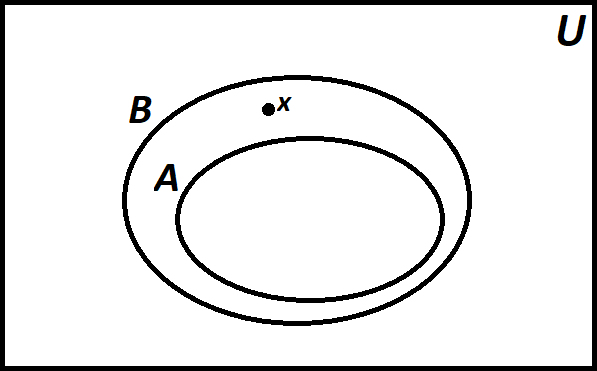
\includegraphics[width = 7.5 cm]{figures/sets/fig-sets-02-00.png}
        \caption{O conjunto $A$ está contido no conjunto $B$, equivalentemente, $B$ contém $A$.}
        \label{fig:sets-02-00}
    \end{figure}

    \textbf{Interseção:} Se estamos interessados em conjuntos/elementos que pertencem simultaneamente a dois conjuntos $A$ e $B$, dizemos que estamos interessados na interseção de $A$ e $B$ (denotada como $A \cap B$)$^{\ref{fig:sets-02-01}}$.
    
    \begin{figure}[hbt!]
        \centering      
        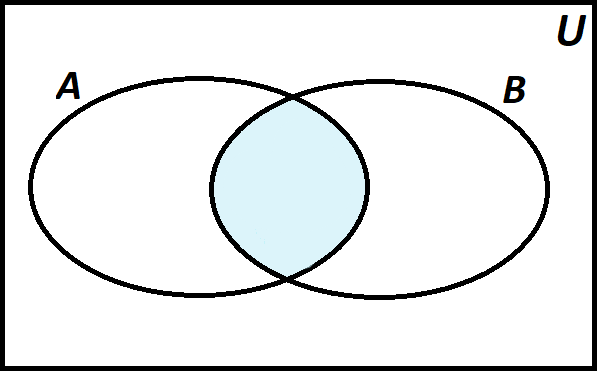
\includegraphics[width = 7.5 cm]{figures/sets/fig-sets-02-01.png}
        \caption{A região azul representa a visualização da interseção dos conjuntos $A$ e $B$.}
        \label{fig:sets-02-01}
    \end{figure}
    
    \textbf{União :}Já se estamos interessados nos conjuntos/elementos que fazem parte de $A$ ou de $B$ dizemos que, nosso objetivo é a união de $A$ e $B$ ($A \cup B$)$^{\ref{fig:sets-02-02}}$.
    
    \begin{figure}[hbt!]
        \centering      
        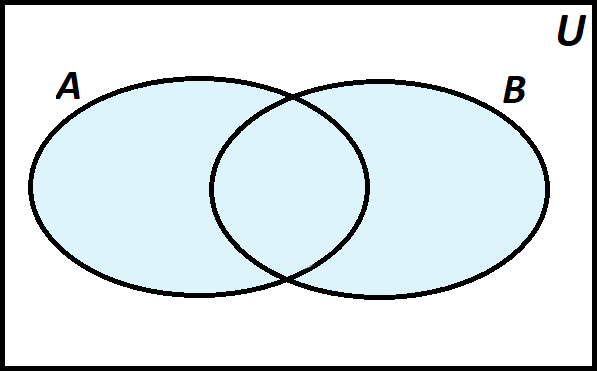
\includegraphics[width = 7.5 cm]{figures/sets/fig-sets-02-02.png}
        \caption{A região azul representa a visualização da união dos conjuntos $A$ e $B$.}
        \label{fig:sets-02-02}
    \end{figure}
    
    \textbf{Universo:} Quando estamos trabalhando com conjuntos é comum definirmos quem é nosso universo ($ \mathcal U $), isto é, o conjunto que conterá todos os conjuntos/elementos que estaremos trabalhando em um contexto$^{\ref{fig:sets-02-03}}$. Por exemplo, na reta real nosso universo é $\mathcal U = \mathbb{R}$.
    
    \begin{figure}[hbt!]
        \centering      
        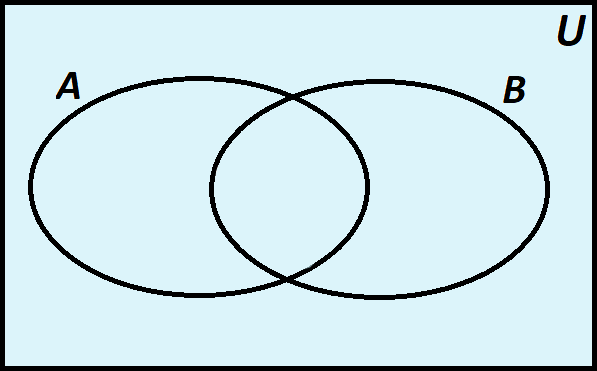
\includegraphics[width = 7.5 cm]{figures/sets/fig-sets-02-03.png}
        \caption{A região azul representa a visualização do nosso Universo.}
        \label{fig:sets-02-03}
    \end{figure}
    
    \textbf{Conjunto Complementar:} Sendo $A$ um conjunto, dizemos que o conjunto $A$ complementar ou complemento de $A$ (denotado como $\overline A$ ou $A^C$)contém todos os conjuntos/elementos que não estão contidos/pertencem a $A$, mas fazem parte de nosso universo ($\mathcal U$)$^{\ref{fig:sets-02-04}}$.
    
    \begin{figure}[hbt!]
        \centering      
        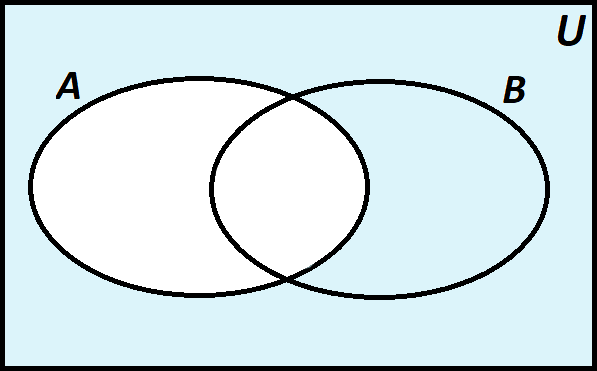
\includegraphics[width = 7.5 cm]{figures/sets/fig-sets-02-04.png}
        \caption{A região azul representa a visualização do complemento de $A$.}
        \label{fig:sets-02-04}
    \end{figure}
    
    \textbf{Diferença de Conjuntos :} Quando temos dois conjuntos e nosso objetivo são os conjuntos/elementos que pertencem a um destes conjuntos, mas não do outro dizemos que estamos interessados na diferença destes conjuntos. No caso, se quero os conjuntos/elementos de $B$, mas não queremos pegar os que também pertencem a $A$, queremos os elementos/conjuntos que pertencem a diferença de $B$ com $A$ (denotamos como $B-A$ ou $B \backslash A$)$^{\ref{fig:sets-02-05}}$.
    
    \begin{figure}[hbt!]
        \centering      
        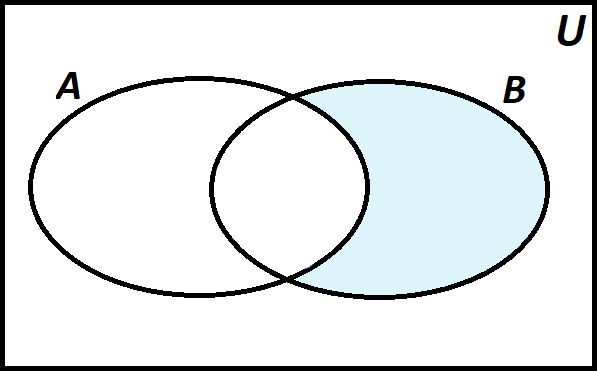
\includegraphics[width = 8 cm]{figures/sets/fig-sets-02-05.png}
        \caption{A região azul representa a visualização da diferença entre os conjuntos $B$ e $A$, isto é, a área onde estão os elementos que pertencem a $B$, mas não pertencem a $A$.}
        \label{fig:sets-02-05}
    \end{figure}
    
    Lembre-se: os diagramas apresentados servem como ferramenta auxiliar para ajudar a entender os conceitos, mas não devem ser vistos como a única ferramenta para compreender as definições e  a teoria exposta.
    
    \newpage
    \subsection{Diagrama de Venn}
    A maneira mais simples de entender a Teoria de Conjuntos, talvez seja o Diagrama de Venn. Criado por John Venn em 1880, esse sistema de representar graficamente conjuntos auxilia imensamente quem está começando a aprender esse assunto, principalmente para entender sobre a parte inicial de notações. Basicamente, consiste em representar num plano, o universo $\mathcal U$ como sendo um retângulo e cada conjunto $A,B,...$ como uma curva fechada simples (geralmente, círculo). Começando com a ideia mais simples, a imagem abaixo representa o conjunto $A$ dentro do univero $\mathcal U$:
    
    %\begin{figure}[h!]
        %\centering
        %\includegraphics{}
        %\caption{Conjunto $A$ dentro de $\mathcal U$}
        %\label{fig:figure_set_01_01}
    %\end{figure}
    
    Para representar que um elemento pertence ao conjunto $A$, simplesmente colocamos ele dentro do espaço delimitado pelo círculo que representa o conjunto, e para representar que um elemento nāo pertence ao conjunto $A$, fazemos o inverso.
    
    
    %\begin{figure}[h!]
    %    \centering
    %    \includegraphics{}
    %    \caption{$a \in A$ e $b \notin A$}
    %    \label{fig:figure_set_01_02}
    %\end{figure}
    
    Quando vamos representar mais de um conjunto em um diagrama de Venn, devemos necessariamente ter todas as possíveis relações, mas o que isso significa? Por exemplo, quando temos $2$ conjuntos $A$ e $B$, significa que devemos ter $4$ regiões representando respectivamente: elementos que pertencem somente à $A$, elementos que pertencem somente à $B$, elementos que pertencem à $A$ e à $B$ simultaneamente e elementos que não pertencem a nenhum dos conjuntos. Precisamos disso, para que tudo que provarmos para dois conjuntos $A$ e $B$, possa ser generalizado para dois conjuntos quaisquer, isso será explicado melhor num exemplo posterior.
    Utilizando esse artífiico, podemos representar todas as definições de intersecçāo, uniāo e diferença de $2$ conjuntos, introduzidas na seçāo anterior, veja nas figuras abaixo:
    
    \subsection{Axiomas}
    
    Agora iremos apresentar alguns axiomas que servirão como base para todo o desenvolvimento dos conteúdos aqui propostos.
    
    \textbf{Axioma da Completude :} Dois conjuntos são iguais, se e somente se, todo elemento que pertence ao primeiro conjunto pertence ao segundo e, todo elemento que pertence ao segundo também pertence ao primeiro, ou seja:
    
    \[\forall A \hspace{1.5mm} \forall B \hspace{1.5mm} (A=B) \iff (\forall x \hspace{1.5mm} (x \in A \iff x \in B))\]
    
    Através desse axioma fica mais claro de entender certa propriedades dos conjuntos. Deste axioma, vem a explicação do motivo de que a ordem dos elementos de um conjunto não importa, pois dado dois conjuntos com os mesmos elemento, mas em ordem diferente (por exemplo, $X=\{a,b,c,d,e,f\}$ e o conjunto $Y=\{e,c,f,b,a,d\}$) eles ainda satisfazem a propriedade de que se $t$ pertence a um deles implica $t$ pertencer ao outro. Outra coisa interessante é que não importa se um conjunto possui elementos repetidos ele continuará igual ao que possui apenas um elemento, isto é, $X=\{a,b,d,e\}$ é igual ao $Y=\{b,a,d,a,e,b,b\}$. Ou seja, em um conjunto não importa a ordem dos elementos, nem as repetições de elementos.
    
    \textbf{Axioma da Existencia do Conjunto Vazio}

\section{Conjuntos em Lean}
    
    Ao longo deste capítulo, observamos que, embora na teoria axiomática dos conjuntos se considere conjuntos de objetos distintos, em matemática é mais comum considerar subconjuntos de algum dominio fixo ($\mathcal U $). É assim que os conjuntos são tratados no Lean. Para qualquer dado do tipo $U$, Lean nos retorna um novo dado tipo $conjunto$ $U$, que consiste nos conjuntos dos elementos de $U$. Assim, por exemplo, podemos raciocinar sobre conjuntos de números naturais, conjuntos de números inteiro ou conjuntos de pares de números naturais.

\subsection{Primeiros Passos}
    Dado $A$ : $set$ $U$ e $x : U$, é possível escrever $x \in A$ para afirmar que $x$ é um elemento do conjunto $A$. O carácter $\in$ pode ser escrito em Lean usando $\backslash$in .
    

\begin{lstlisting}

import data.set
    open set

    variable {U : Type}
    variables A B C : set U
    variable x : U

    #check x ∈ A
    #check A ∪ B
    #check B \ C
    #check C ∩ A
    #check -C
    #check ∅ ⊆ A
    #check B ⊆ univ
    
 \end{lstlisting}


Abaixo temos uma pequena lista de como se representa os principais caractéres da parte de conjuntos no Lean: 

\begin{itemize}
    \item $\in$ $\rightarrow$ $\backslash$in
    \item $\notin$ $\rightarrow$ $\backslash$notin
    \item $\subset$ $\rightarrow$ $\backslash$subset
    \item $\subseteq$ $\rightarrow$ $\backslash$sub
    \item $\emptyset$ $\rightarrow$ $\backslash$empty
    \item $\cup$ $\rightarrow$ $\backslash$un \ ou \ $\backslash$cup \ ou \ $\backslash$union
    \item $\cap$ $\rightarrow$ $\backslash$i \ ou \ $\backslash$cap \ ou \ $\backslash$intersction
\end{itemize}
Obs$^{1}$.: O conjunto universal é denotado $univ$.

Obs$^{2}$.: O complementar de um conjunto é denotada com um símbolo de negação antes de seu símbolo, assim: 

Noções básicas da teoria dos conjuntos são definidas na biblioteca principal do Lean, mas teoremas e notações adicionais estão disponíveis em uma biblioteca auxiliar que é carregada com o comando import data.set, que deve aparecer no início do arquivo.

\chapter{Relações}
Em capítulos anteriores, discutimos proposições que lidavam com a relação entre objetos matemáticos. Muitas vezes na matemática, e mesmo no contexto em que estamos inseridos, estamos interessados em definir e estudar relações entre objetos distintos. Por exemplo, podemos estar interessados em certas própriedades sobre a relação \textit{é vais velho que}, entre seres vivos, e diremos que essa é uma relação \textit{irreflexiva}, \textit{transitiva}, ou ainda, uma relação de \textit{ordem estrita}.

Nesse capítulo discutimos exatamente essas noções, e definimos certos tipos de relaçõs mais comuns.

\section{Semântica das Relações}
Podemos abstrair a noção semântica de relação para um universo $R$ de tuplas de aridade definida, que contem a sequencia dos objetos relacionados. Por exemplo, considere que o elemento $a$ está relacionado a $b$ por uma relação $R$. Ppodemos denotar $aRb$, ou $R(a,b)$ significando que o par $(a,b)\in R$, está definido como existente no universo daquela relação. Como se pode esperar, a relação pode ter qualquer aridade necessária, e relacionar objetos de tipos distintos.

Considere, a partir disso, o universo de objetos $u = \{Ana, Bia, Cid\}$, e a relação \textit{conhece}, definida por $U\times U \supseteq A = \{(Ana, Bia), (Bia, Cid)\}$. Podemos dizer que \textit{Bia conhece Ana}?

\section{Definições}
Iniciamos a seção propondo uma série de definições de relações extremamente úteis a partir das próximas subseções.

\subsection{Relações de Ordem}
Definições usando $\leq$ e o $<$... Podemos definir uma relação estrita por uma parcial, e uma parcial por uma estrita... etc. Algum exemplo não numérico!

\subsection{Relações de Equivalência}
Descrevemos as propriedades que definem esse tipo de relação, e damos exemplos. Mostramos as notações $a\sim b $, $a\equiv b$. Sugiro as relações de equivalencia "paralelo a", "modulo n", "mesma idade".

\subsection{Equivalencia e Igualdade}
Apenas discutimos brevemente como e porque Equivalencia e Igualdade são animais completamente diferentes. Toma os exemplos acima pra discutir.

\section{Relações em Lean}

\section{Exercícios}

\chapter{Funções}

Desde o final do século XIX, diversas áreas da matemática
estudam consistentemente \textit{\hyperlink{chapter.4}{conjuntos}},
\textit{\hyperlink{chapter.5}{relações}}, já apresentadas
nesse texto, e funções. Neste capítulo, debruçaremos nossa
atenção nas propriedades dessa terceira área.

Entende-se que uma função $f$ é um mapeamento entre um
domínio $X$ e um domínio $Y$, este que será conhecido como
contradomínio, posteriormente. Entretanto, para teóricos
de conjuntos, esses domínios são simplesmente considerados
conjuntos. Vimos que \textit{\hyperlink{chapter.2}{Lean}} é uma
linguagem baseada em Tipos. Dessa forma, estabelece-se uma
diferença clara entre o Domínio $X$, caracterizado pelos Tipos, e
o Conjunto $A$, que é do tipo (sub)conjunto de $X$. Em Lean:
\begin{lstlisting}
variable X : Type
variable A : set X
\end{lstlisting}

Entretanto a visão da função como mapeamento entre conjuntos
é comum entre os matemáticos e será considerada nesse texto,
fazendo as devidas comparações com a linguagem de referência,
o Lean.

\section{O Conceito de Função}

Considere dois conjuntos quaisquer $X$ e $Y$ e um mapeamento $f$
do conjunto $X$ para o conjunto $Y$. Se $f$ atribui um e apenas
um valor para cada elemento de $X$, dizemos que $f$ é uma função total, e
escrevemos $f: X \to Y$.  Chamamos $X$ de domínio de $f$, enquanto
$Y$ é o contradomínio de $f$ e $\forall x, (x \in X  \Rightarrow f(x) \in Y)$.
Nesse sentido, $\forall x_1 \in X, \forall x_2 \in X, x_1 = x_2 \Rightarrow f(x_1) = f(x_2)$.
Uma função também pode ser parcial quando ela não é definida para alguns valores
do domínio. Como toda função parcial é total ao restringir o domínio, trateremos
nesse texto das funções totais.

A maneira mais simples de se representar uma função é escrevê-la explicitamente
para cada elemento do domínio. Por exemplo, podemos escrever as seguintes expressões:

\begin{itemize}
    \item Seja $f: \mathbb{N} \to \mathbb{N}$ definida por
    $f(n) = 2\cdot n + 1$
    \item Seja $g : \mathbb{N} \to \mathbb{R}$ definida por
    $g(n) = \frac{n}{n+1}$
    \item Seja $h : \mathbb{R} \to \{0,1\}$ definida por
    $$\left \{ \begin{array}{c}
    h(x) = 1 ~if~x \in \mathbb{Q} \\
    h(x) = 0 ~ if ~ x \not \in \mathbb{Q} \\
    \end{array}
    \right. $$
 \end{itemize}

A questão que se levanta é: o que torna uma expressão explícita legítima?
Neste momento, deixaremos essa questão de lado e notaremos que a matemática
é confortável com diversos tipos de definições, como, por exemplo, a definição
de $h(x)$ no exemplo acima. Nesse mesmo exemplo, não fica claro em como podemos
definir algoritmicamente se um número real de entrada é um número racional ou não.
Porém, esse não é o objetivo do capítulo.

Note que a escolha das variáveis $x$ e $n$ são arbitrárias.
Isto nos leva à definição no capítulo de \textit{\hyperlink{chapter.4}{FOL}} de
variável ligada (\textit{bound}), visto que se renomearmos $x$ com $y$, os valores
continuam os mesmos.

Lógicos frequentemente utilizam a notação $\lambda x e(x)$ para denotar a função
que mapeia $x$ para $e(x)$. Essa notação chama-se \textit{notação lambda} e pode
ser usada da seguinte forma: $f = \lambda x(x + 1)$, que significa $f(x) = x + 1$.
Essa notação é mais interessante para cientistas da computação e lógicos do que
propriamente para matemáticos. Em Lean, definimos da seguinte forma:

\begin{lstlisting}
variables X Y : Type
variable f : X → Y
\end{lstlisting}

Lembre-se que diferenciamos o tipo $X$ do tipo $set~X$ em Lean.

\section{Primeiras Definições}

\theoremstyle{definition}
%\newtheorem{definition}{Definição}[section]

\theoremstyle{definition}
\newtheorem{example}{Exemplo}[section]

\theoremstyle{plain}
%\newtheorem{theorem}{Proposição}[section]

\theoremstyle{plain}
\newtheorem{corollary}{Corolário}[section]

\begin{definition}
    \label{def1}
    Seja um conjunto $X$. A função identidade de $A$ é a função
    $i_A : A \rightarrow A$ definida para todos os valores $x \in A$ tal que $i_A(x) = x$.
\end{definition}

\begin{definition}
    \label{def2}
    Sejam $f : X \rightarrow Y$ e $g : Y \rightarrow Z$ funções.
    Defina $k : X \rightarrow Z$ por $k(x) = g(f(x))$. A função $k$ é chamada de composição
    de $f$ e $g$ ou $f$ composta com $g$ e é escrita $g \circ f$. Desta forma, para cada elemento,
    primeiro  avaliamos $f(x) \in Y$ e depois avaliamos $g(f(x)) \in Z$.
\end{definition}

Podemos ver em Lean as definições de composição e de identidade. Note que estamos em um namespace
hidden para que não haja conflito de definições.

\begin{lstlisting}
namespace hidden
    variables {X Y Z : Type}

    def comp (f : Y → Z) (g : X → Y) : X → Z :=
    λx, f (g x)

    infixr  ` ∘ ` := comp

    #check @comp

    def id (x : X) : X := x

    #check @id

end hidden
\end{lstlisting}

\begin{definition}
    \label{def3}
    Considere $f,g : X \to Y$. Dizemos que essas funções são iguais,
    quando para todos os valores do domínio $X$, a correspondência no contradomínio $Y$ é a
    mesma. Em lógica simbólica, $\forall x (x \in X \to (f(x) = g(x)) \iff f = g $.
\end{definition}

Obseve que em termos de lógica formal de tipos, poderíamos reescrever como
$\forall x : X (f(x) = g(x)) \iff f = g$. Escrevemos essa equivalência entre lógica e funções
utilizando a extensionalidade das funções, muito semelhante à descrita no capítulo de
\textit{\hyperlink{chapter.5}{conjuntos}}. Por exemplo, se $f, g : \mathbb{R} \to \mathbb{R}$
definidas por $f(x) = x + 1$ e $g(x) = 1 + x$, então $f = g$, pois para cada valor de $x$, vale
a comutativade da soma.

Em lean, o comando \lstinline{funext} (de "function extensionality") prova a igualdade de funções.

\begin{lstlisting}
variables {X Y : Type}

example (f g : X → Y) (h : ∀ x, f x = g x) : f = g :=
    funext h
\end{lstlisting}

\begin{theorem}
    \label{prop1}
    Para todo $f: X \to Y$, $f \circ i_X = f$ e $i_Y \circ f = f$
\end{theorem}
\begin{proof}
    Seja $x$ um elemento qualquer de $X$. Então $(f \circ i_X)(x) = f(i_X(x)) = f(x)$
     e $(i_Y \circ f)(x) = i_Y(f(x)) = f(x)$, o que mostra a igualdade.
\end{proof}

No Lean, podemos mostrar essa proposição da seguinte forma. Para algumas funções, será necessário
escrevermos \lstinline{open function}.

\begin{lstlisting}
variables {X Y Z W : Type}

lemma left_id (f : X → Y) : id ∘ f = f := rfl

lemma right_id (f : X → Y) : f ∘ id = f := rfl

theorem comp.assoc (f : Z → W) (g : Y → Z) (h : X → Y) :
    (f ∘ g) ∘ h = f ∘ (g ∘ h) := rfl

\end{lstlisting}

\begin{definition}
    \label{def4}
    Suponha $f:X \to Y$ e $g : Y \to X$ satisfaz $g \circ f = i_X$. Assim,
    $g(f(x)) = i_X(x) = x$, para todos os elementos de $X$. Neste caso $g$ é dita inversa à esquerda
    de $f$ e $f$ é dita inversa à direita de $g$. Quando $g$ é inversa à direita e é inversa à esquerda
    de $f$, então $g$ é dita simplesmente inversa de $f$.
\end{definition}

\begin{example}
    \label{ex1}
    Defina $f,g : \mathbb{R} \to \mathbb{R}$ por $f(x) = x + 1$ e $g(x) = x - 1$. Então $g$
    é inversa à direita e à esquerda de $f$ e vice-versa.
\end{example}
\begin{example}
    \label{ex2}
    $\mathbb{R}^{+}$ denota os reais não negativos. Defina $f : \mathbb{R} \to \mathbb{R}^{+}$
    por $f(x) = x^2$ e defina $g : \mathbb{R}^2 \to \mathbb{R}$ por $g(x) = \sqrt{x}$. Então
    $f(g(x)) = (\sqrt{x})^2 = x$, para todo $x$ no domínio de $g$. Então $f$ é inversa à esquerda de $g$
    e $g$ inversa à direita de $f$. Por outro lado, $g(f(x)) = \sqrt{x^2} = |x|$. Logo $g$ não é inversa à
    esquerda de $f$ e $f$ não é inversa à direita de $g$.
\end{example}

\begin{theorem}
    \label{prop2}
    Suponha que $f : X \to Y $ tem inversa à esquerda, $h : Y \to X $ e uma inversa à direita, $k : Y \to X $.
    Então $h = k$.
\end{theorem}
\begin{proof}
    Seja $y \in Y$. $h(f(k(y))) = k(y)$, pois $h$ é uma inversa à esquerda de $f$.
    Por outro lado, $f(k(y)) = y$ e, portanto $h(f(k(y))) = h(y)$. Assim $k(y) = h(y) $ e as funções são iguais.
\end{proof}

Essa proposição pode também ser vista em Lean. Considerarei a prova utilizando táticas. O leitor pode estudar
aquela que sentir mais confortável. Note que neste exemplo, já foi necessário o \lstinline{namespace function},
visto que \lstinline{left_inverse} e \lstinline{right_inverse} já estão predefinidas.

\begin{lstlisting}
open function

variables {X Y Z: Type}

-- Term and Calc Mode
example (f: X → Y) (h: Y → X) (k: Y → X)
    (hf: left_inverse h f) (fk: right_inverse k f): h = k :=
    have H: ∀ ( x : Y ), h x = k x, from
        assume x,
        have h1: h (f (k x)) = k x , from calc
            h ( f (k x)) = k x: by apply hf,
        have h2: h (f (k x)) = h x, from calc
            h (f (k x)) = h x: by rw fk,
        show h x = k x, from eq.trans (eq.symm h2) h1,
    show h = k, from funext H

-- Tatics Mode
example (f: X → Y) (h: Y → X) (k: Y → X)
    (hf: left_inverse h f) (fk: right_inverse k f): h = k :=
    begin
        apply funext,
        assume x,
        have hf: h (f (k x)) = k x, by apply hf,
        rw ←hf,
        rw fk,
    end
\end{lstlisting}

\begin{theorem}
    \label{prop3}
    Seja $f: X \to Y$. Se a inversa de $f$ existe, então ela é única. Isto é, se $g_1, g_2: Y \to X$ são inversas
    de $f$, então $g_1 = g_2$
\end{theorem}
\begin{proof}
    Sabemos que $g_1$ é inversa à esquerda de $f$. Então,
    $$g_1(f(g_2(x))) = g_2(x), ~para~todos~os~valores~de~x.$$
    Também, $g_2$ é inversa de $f$. Então,
    $$g_1(f(g_2(x))) = g_1(x), ~para~todos~os~valores~de~x.$$ Logo $g_1 = g_2$.
\end{proof}

Quando a inversa de $f$ existe, então, podemos escrevê-la como $f^{-1}$. Dada a Definição \hyperlink{def4},
podemos afirmar que $(f^{-1})^{-1} = f$.

Observe que uma função pode possuir mais de uma função inversa à esquerda ou mais de uma função inversa
à direita. Ainda, quando uma função possui mais de uma função inversa à esquerda, ela não possui inversa
à direita. Se ela possuisse, ela seria igual a todas as funções inversas à esquerda pela Proposição \ref{prop2},
portanto elas seriam iguais, o que é uma contradição, por hipótese. O mesmo vale para inversas à direita.

\begin{theorem}
     \label{prop4}
     Seja $f: X \to Y $ e $g: Y \to Z$. Se $h: Y \to X$ e $k: Z \to Y$ são inversas à esqueda de $f$ e $g$,
     respectivamente, então $h \circ k$ é inversa à esquerda de $g \circ f$. O mesmo vale quando substituimos
     esquerda por direita na proposição.
\end{theorem}

\begin{proof}
 $(h \circ k)\circ(g \circ f)(x) = h(k(g(f(x)))) = h(f(x)) = x $. A demonstração quando substituimos a proposição
 de esquerda para direita é análoga e é deixada como exercício ao leitor.
\end{proof}

\begin{corollary}
    \label{cor1}
    Se $f: X \to Y$ e $g: Y \to Z$ possuem inversas, então $(f \circ g)^{-1}$ existe e
    $(f \circ g)^{-1} = f^{-1} \circ g^{-1}$.
\end{corollary}

\begin{proof}
    Segue diretamente da Proposição \ref{prop4} e Proposição \ref{prop2}.
\end{proof}

\section{Funções Injetiva, Sobrejetiva e Bijetiva}

\begin{definition}[Função Injetiva]
    \label{def5}
    Também conhecida como função injetora, é uma função em que elementos distintos do domínio são
    mapeados para elementos diferentes do contradomínio. Dessa forma, seja $f: X \to Y$. Se
    $\forall x_1 \in X, \forall x_2 \in X, x_1 \neq x_2 \Rightarrow f(x_1) \neq f(x_2) $, f é injetiva.
    A definição pode ser feita pela contrapositiva dessa afirmação, também. A definição pela contrapositiva
    será bastante utilizada nas demonstrações.
\end{definition}

\begin{definition}[Função Sobrejetiva]
    \label{def6}
    Também conhecida como função bijetora, é uma função em que todos os elementos do contradomínio
    estão na imagem da função. Dessa forma, seja $f: X \to Y$. Se $\forall y \in Y, \exists x \in X, f(x) = y$,
    f é sobrejetiva.
   \end{definition}

\begin{definition}[Função Bijetiva]
    \label{def7}
    Também conhecida como bijeção ou correspondência um a um, é uma função simultaneamente injetiva e
    sobrejetiva.
\end{definition}

Em Lean, essas definições são descritas no \lstinline{namespace function}.

\begin{example}
    Considere $X = {1,2,3,4}$ e $Y = \{John, Paul, George, Ringo\}$. É possível construir uma função bijetiva
    entre o conjunto $X$ e o conjunto $Y$.
\end{example}

\begin{lstlisting}
variables {X Y: Type}

def injective (f : X → Y) : Prop :=
∀ x₁ x₂, f x₁ = f x₂ → x₁ = x₂

def surjective (f : X → Y) : Prop :=
∀ y, ∃ x, f x = y

def bijective (f : X → Y) := injective f ∧ surjective f
\end{lstlisting}

\begin{theorem}
    \label{prop5}
    Seja $f : X \to Y$.
    \renewcommand{\labelenumi}{\Roman{enumi}}
    \begin{enumerate}
        \item Se $f$ possui inversa à esquerda, $f$ é injetiva.
        \item Se $f$ possui inversa à direita, $f$ é sobrejetiva.
        \item Se $f$ possui inversa, $f$ é bijetiva.
    \end{enumerate}
\end{theorem}
\begin{proof}
    Para provar I), suponha que $f(x_1) = f(x_2)$ e que $g$ é inversa à esquerda
    de $f$. Assim $g(f(x_1)) = x_1$ e $g(f(x_2)) = x_2)$. Portanto $x_1 = x_2$ e
    está provado. Para provar II), considere $h$ inversa à direita de $f$. Seja
    $y \in Y$ e $x = h(y)$. Então $f(x) = f(h(y)) = y$. A terceira sai diretemente
    das duas anteriores.
\end{proof}

\begin{lstlisting}
open function

variables {X Y : Type}

theorem inj_of_left_inverse {g : Y → X} {f : X → Y} :
left_inverse g f → injective f :=
    assume h, assume x₁ x₂, assume feq,
    calc x₁ = g (f x₁) : by rw h
        ... = g (f x₂) : by rw feq
        ... = x₂       : by rw h

theorem surj_of_right_inverse {g : Y → X} {f : X → Y} :
right_inverse g f → surjective f :=
    assume h, assume y,
    let  x : X := g y in
    have f x = y, from calc
        f x  = (f (g y))    : rfl
        ... = y            : by rw [h y],
    show ∃ x, f x = y, from exists.intro x this
\end{lstlisting}

\begin{theorem}
    \label{prop6}
    Seja $f: X \to Y$
    \renewcommand{\labelenumi}{\Roman{enumi}}
    \begin{enumerate}
        \item Se $X$ é não vazio e $f$ é injetiva, então $f$ possui inversa à esquerda.
        \item Se $f$ é sobrejetiva, então $f$ possui inversa à direita.
        \item Se $X$ é não vazio e $f$ é bijetiva, então $f$ possui inversa.
    \end{enumerate}
\end{theorem}

\begin{proof}
    Seja $\hat{x} \in X$. Defina uma função $g: Y \to X$ com $g(y) = x$, tal que $f(x) = y$,
    caso exista esse $x$. Caso ele não exista, $g(y) = \hat{x}$. Agora, suponha que
    $g(f(x)) = x'$. Pela definição de $g$, $f(x) = y$, logo $g(y) = x$. Assim, $f(x) = f(x')$.
    Como $f$ é injetiva $x = x'$.

    Para a segunda afirmação, defina $h: Y \to X$, onde, para cada $y \in Y$, escolha um elemento
    $x \in X$, tal que $h(y) = x$. Note que a sobrejetividade garante a existência desse elemento,
    mas não garante a unicidade. Então $f(h(y)) = f(x) = y$, por definição de $h$.

    A fim de provar a terceira, basta as demonstrações das anteriores.
\end{proof}

Algumas observações sobre essa demonstração são importantes. Ao definir $g$ na primeira parte,
precisa-se decidir se $x \in X$ existe tal que $f(x) = y$. Isso pode não ser algoritmicamente
feito, logo $g$ poderia não ser computável. Na construção de $h$, a prova requere que haja
uma escolha de valor de $x$ entre os possíveis candidatos. Isto é uma versão do
\href{https://pt.wikipedia.org/wiki/Axioma_da_escolha#Enunciado}{\textit{axioma da escolha}}.
Este axioma foi muito debatido no século XX, mas hoje já é comum para demonstrações. O paradoxo
de Banach-Tarski é um argumento contra o axioma.

Utilizando conceitos e resultados da seção anterior, podemos provar a seguinte proposição.

\begin{theorem}
    Seja $f: X \to Y$ e $g: Y \to Z$.
    \renewcommand{\labelenumi}{\Roman{enumi}}
    \begin{enumerate}
        \item Se $f$ e $g$ são injetivas, $g \circ f$ também será.
        \item Se $f$ e $g$ são sobrejetivas, $g \circ f$ também será.
    \end{enumerate}
\end{theorem}

\begin{proof}
    Basta aplicarmos a Proposição \ref{def4} e definirmos $h$ e $k$ como
    inversas à esquerd ade $f$ e $g$ respefticamente. Logo $(h \circ k)$
    é inversa à esquerda de  $(g \circ f)$ e, portanto, ela é injetiva.

    O mesmo vale para a segunda afirmação.
\end{proof}

\begin{lstlisting}
open function

namespace hidden
    variables {X Y Z : Type}

    theorem injective_comp {g : Y → Z} {f : X → Y}
    (Hg : injective g) (Hf : injective f) :
    injective (g ∘ f) :=
        assume x₁ x₂,
        assume : (g ∘ f) x₁ = (g ∘ f) x₂,
        have f x₁ = f x₂, from Hg this,
        show x₁ = x₂, from Hf this

    theorem surjective_comp {g : Y → Z} {f : X → Y}
        (hg : surjective g) (hf : surjective f) :
    surjective (g ∘ f) :=
    begin
        assume z,
        apply exists.elim (hg z),
        assume y (hy: g y = z),
        apply exists.elim (hf y),
        assume x (hx: f x = y),
        rw ←hx at hy,
        apply exists.intro x hy
    end

    theorem bijective_comp {g : Y → Z} {f : X → Y}
        (hg : bijective g) (hf : bijective f) :
        bijective (g ∘ f) :=
    have ginj : injective g, from hg.left,
    have gsurj : surjective g, from hg.right,
    have finj : injective f, from hf.left,
    have fsurj : surjective f, from hf.right,
    and.intro (injective_comp ginj finj)
                (surjective_comp gsurj fsurj)
end hidden
\end{lstlisting}

\begin{example}
    Considere $f: \mathbb{N} \to Y$, tal que $f(n) = 2n$. Podemos, ter:
    \begin{itemize}
        \item $Y = \mathbb{N}$. $f$ é injetiva, mas não é sobrejetiva.
        \item $Y = \mathbb{R}$. $f$ é injetiva, mas não é sobrejetiva.
        \item $Y = \{n \in \mathbb{N} | n~par\}$. $f$ é bijetiva.
    \end{itemize}
\end{example}

\section{Funções e Subconjuntos do Domínio}

Nós podemos querer saber o comportamento de uma função em algum subconjunto
$A$ de  $X$. Por exemplo, podemos dizer que $f$ é injetiva em $A$ se para
todo $x_1$ e $x_2$ em A, $f(x_1) = f(x_2) $ implicar $x_1 = x_2 $.

\begin{definition}
    \label{def8}
    Se $f$ é função de $X$ e $Y$, dizemos que $f[A]$ denota a imagem de $f$ em
    $A$, definido por $f[A] = \{y \in Y | ~\exists x \in A, y = f(x)\}$.
\end{definition}

\begin{theorem}
    \label{prop7}
    Seja $f: X \to Y $ e $A$ um subconjunto de $X$. Então, para todo $x$ em
    $A$, $f(x)$ está em $f[A]$.
\end{theorem}

\begin{proof}
    Por definição, $f(x) \in f[A] $ se, e somente se, existe $x'$ em $A$ tal que
    $f(x') = f(x)$. Isto vale para  $x' = x $.
\end{proof}

\begin{theorem}
    \label{prop8}
    Seja $f: X \to Y$ e $g: Y \to Z$. Seja $A$ subconjunto de $X$. Então
    $$(g \circ f)[A] = g[f[A]]$$
\end{theorem}

\begin{proof}
    Seja $z \in (g \circ f)[A]$. Então, para algum $x \in A$, $z = (g \circ f)(x) = g(f(x))$.
    Pelo que acabamos de provar na Proposição \ref{prop8}, $f(x) \in f[A]$. Novamente, pelo
    que acabamos de provar, $g(f(x)) \in g[f[A]] $.

    Alternativamente, seja $z \in g[f[A]]$. Então, existe $y$ em $f[A]$ tal que
    $f(y) = z$. Como $y \in f[A]$, existe $x \in A$, tal que $f(x) = y$. Então
    $(g \circ f)(x) = g(f(x)) = g(y) = z$, então $z \in (g \circ f)[A] $
\end{proof}

Uma prova de que a composição de funções sobrejetivas é
sobrejetiva é a que descrevemos cima, pois $f: X \to Y$ é
sobrejetiva se, e somente se, $f[X] = Y$.

Nós podemos ver $f$ como uma função de $A$, um subconjunto de $X$ a $Y$, simplesmente
ignorando o comportamento de $f$ nos elementos fora de $A$.

\begin{definition}
    \label{def9}
    Denotamos $f \upharpoonright A$ como restrição de $f$ para $A$. Isto é, dadas $f: X \to Y$
    e $A \subseteq X$, $f \upharpoonright A : A \to Y$ é definida por $(f \upharpoonright A)(x) = x$,
    para todo $x$ em $A$.
\end{definition}

Agora, $f$ é injetiva em $A$ significa que a restrição de $f$ em $A$ é injetiva.

\begin{definition}[Pré-imagem]
    \label{def10}
    Se $f: X \to Y$ e $B \subseteq Y$, então a pré-imagem de $B$ em $f$, denotado por $f^{-1}[B]$ é
    definida por $f^{-1}[B] = \{x \in X | f(x) \in B\}$. Ou seja, é o conjunto de elementos de $X$ que
    são mapeados em $B$.
\end{definition}

Note que essa definição faz sentido mesmo que $f$ não tenha inversa, visto que dado $y \in B$ pode não
haver $x \in X$ com a propriedade de $f(x) \in B$, como podem ter vários. Se $f$ tem inversa ($f^{-1}$),
então, para todo $y$ em $B$, existe exatamente um elemento $x$ em $X$ com $f(x) \in B$. Neste caso,
dizemos que $f^{-1}[B]$ é a imagem de $B$ sobre $f^{-1}$ ou a pré-imagem de $B$ sobre $f$.

\begin{theorem}
    Seja $f: X \to Y$, $g: Y \to Z$ e $C \subseteq Z$. Então $$(g \circ f)^{-1}[C] = f^{-1}[g^{-1}[C]]$$.
\end{theorem}
\begin{proof}
    Para qualquer $y$, $y \in (g \circ f)^{-1}[C]$ se, e somente se, $g(f(y))$ está em $C$.
    Isto acontece se, e somente se, $f(y) \in g^{-1}[C]$, o que acontece se, e somente se $y \in f^{-1}[g^{-1}[C]]$.
\end{proof}

Seguem algumas propriedades sobre imagens e pré-imagens. Aqui, $f$ denota uma função
arbitrária de $X$ em $Y$. $A, A_1, A_2, ...$ denotam subconjuntos arbitrários de $X$,
e $B, B_1, B_2,...$ denotam subconjuntos arbitrários de $Y$.

\begin{enumerate}
    \item $A \subseteq f^{-1}[f[A]]$, e se $f$ é injetiva, $A = f^{-1}[f[A]]$.
    \item $f[f^{-1}[B]] \subseteq B$, e se $f$ é sobrejetiva, $B = f[f^{-1}[B]]$.
    \item Se $A_1 \subseteq A_2$, então $f[A_1] \subseteq f[A_2]$.
    \item Se $B_1 \subseteq B_2$, então $f^{-1}[B_1] \subseteq f^{-1}[B_2]$.
    \item $f[A_1 \cup A_2] = f[A_1] \cup f[A_2]$.
    \item $f^{-1}[B_1 \cup B_2] = f^{-1}[B_1] \cup f^{-1}[B_2]$.
    \item $f[A_1 \cap A_2] \subseteq f[A_1] \cap f[A_2]$ e, se $f$ é injetiva, $f[A_1 \cap A_2] = f[A_1] \cap f[A_2]$.
    \item $f^{-1}[B_1 \cap B_2] = f^{-1}[B_1] \cap f^{-1}[B_2]$.
    \item $f[A] \setminus f[B] \subseteq f[A\setminus B]$.
    \item $f^{-1}[A] \setminus f^{-1}[B] \subseteq f[A \setminus B]$.
    \item $f[A] \cap B = f[A \cap f^{-1}[B]]$.
    \item $f[A \cup f^{-1}[B]] \subset f[A] \cup B $.
    \item $A \cap f^{-1}[B] \subseteq f^{-1}[f[A] \cap B]$.
    \item $A \cup f^{-1}[B] \subseteq f^{-1}[f[A] \cup B]$.
\end{enumerate}

A partir de agora, vamos demonstrar algumas dessas proporições, ora
com descrições da demonstração e ora com provas em Lean. Tambémm sugerimos
que essas proposições sejam exercícios para a leitora ou o leitor.

\subsection{Demonstrações com linguagem natural}

\begin{theorem}[Item 7]
    \label{exerc1}
    Sejam $X$ e $Y$ conjuntos, $A_1, A_2 \in X$ e $f: X \to Y$.
\end{theorem}

\begin{proof}
    Se $y \in f[A_1 \cap A_2]$, temos que existe $x \in A_1 \cap A_2$, com $f(x) = y$.
    Nesse caso, $f(x) \in f[A_1]$, e $f(x) \in f[A_2]$, o que demonstra a primeira parte.

    Agora, suponha a injetividade de $f$. Suponha também que $y \in f[A_1] \cap f[A_2]$. Assim, existem
    $x_1 \in A_1$ e $x_2 \in A_2$, com as propriedades de $f(x_1) = y = f(x_2)$. Como a função é injetiva,
    $f(x_1) = f(x_2) \Rightarrow x_1 = x_2$. Assim $x_1 \in A_2$, que implica $x_1 \in A_1 \cap A_2$. Logo,
    $y \in f[A_1 \cap A_2]$.
\end{proof}

\begin{theorem}[Item 11]
    \label{exerc2}
    Sejam $X$ e $Y$ conjuntos, $f: X \to Y, A \subseteq X$ e $B \subseteq Y$. Então,
    $f[A] \cap B = f[A \cap f^{-1}[B]]$
\end{theorem}

\begin{proof}
    Suponha, inicialmente, que $y \in f[A] \cap B$. Então $y \in B$ e para algum $x \in A$, $f(x) = y$.
    Nesse sentido, $x \in f^{-1}[B]$. Assim, $x \in A \cap f^{-1}[B]$ e, portanto, $y \in f[A \cap f^{-1}[B]]$.

    Alternativamente, se $y \in f[A \cap f^{-1}[B]]$, existe $x \in A \cap f^{-1}[B]$, com $f(x) = y$.
    Daqui, concluímos que $y = f(x) \in f[A]$ e $y \in B$, pela definição de pré-imagem. Então $y \in f[A] \cap B$,
    como queríamos provar.
\end{proof}

\subsection{Demontrações em Lean}

Nós podemos utilizar variáveis limitadas para falar sobre o comportamento de funções
em conjuntos particulares.

\begin{lstlisting}
import data.set -- inclui o símbolo de subconjunto da imagem ''
open set function

variables {X Y : Type}
variables (A  : set X) (B : set Y)

def maps_to (f : X → Y) (A : set X) (B : set Y) :=
    ∀ x ∈ A, f x ∈ B

def inj_on (f : X → Y) (A : set X) :=
    ∀ (x₁ ∈ A) (x₂ ∈ A), f x₁ = f x₂ → x₁ = x₂

def surj_on (f : X → Y) (A : set X) (B : set Y) :=
    B ⊆ f '' A

\end{lstlisting}

A definição de \lstinline{maps_on} é a ideia de que a imagem de um subconjunto do
domínio $X$ está totamente inclusa em um subconjunto específico do contradomínio. As
definições de \lstinline{inj_on} e \lstinline{surj_on} são as definições usuais.

\begin{theorem}[Item 3]
\end{theorem}

\begin{theorem}[Item 9]
\end{theorem}

Observe que para o item 9, trataremos $X$ e $Y$ como conjuntos iguais. Caso não sejam,
$f[B]$ pode nem estar definida.

\begin{lstlisting}
import data.set
open set function

variables {X Y : Type}
variables (A B A₁ A₂ : set X)

theorem item3 (f: X → Y) : A₁ ⊆ A₂ → f '' A₁ ⊆ f '' A₂ :=
    assume h : A₁ ⊆ A₂,
    assume y,
    assume h₁ : y ∈ f '' A₁,
    have h₂ : ∃ x, x ∈ A₁ ∧ f(x) = y, from h₁,
    show y ∈ f '' A₂, from exists.elim h₂
        (assume (x' : X) (ha: x' ∈ A₁ ∧ f(x') = y ),
        have h₃ : x' ∈ A₂ ∧ f(x') = y, from and.intro (h ha.left)  ha.right,
        show y ∈ f '' A₂, from exists.intro x' h₃)

theorem item9 (f: X → X) : f '' A \ f '' B ⊆ f '' (A \ B) :=
begin
    intros y h,
    have h₁ : y ∈ f '' A, from mem_of_mem_diff h,
    have h₂ : ¬ (y ∈ f '' B), from not_mem_of_mem_diff h,
    apply exists.elim h₁,
    intros x h₃,
    apply exists.intro x,
    apply and.intro,
    apply mem_diff_of_mem,
        exact h₃.left,
        assume h₄ : x ∈ B,
        exact false.elim (h₂ (exists.intro x (and.intro h₄ h₃.right))),
        exact h₃.right
end

#check @mem_of_mem_diff
#check @not_mem_of_mem_diff
#check @mem_diff_of_mem

\end{lstlisting}

As funções \lstinline{mem_of_mem_diff, not_mem_of_mem_diff} e \lstinline{mem_diff_of_mem}
tem o objetivo de lidar com a diferença esua relação com a interseção. Note que usar táticas
auxilia o passo a passo, porém dificulta o posterior entendimento. Por isso, é recomendável,
nesses exemplos, utilizar alguma ferramenta para Lean. 
Essas funções e outras já apresentadas, encontram-se na biblioteca do Lean e grande parte delas está 
disponível quando você abre o namespace \lstinline{function}.

\begin{lstlisting}
open function 

#check @comp 
#check @has_left_inverse
-- A right_inverse tem duas definicoes para Lean. Apenas uma
-- esta no namespace function. Por isso e importante especificar. 
#check @function.right_inverse    
\end{lstlisting}

\section{Lógica de Segunda ou Mais Alta Ordem}

Até agora, formalmente, definimos lógica de primeira ordem, onde iniciamoscom um estoque 
fixo de símbolos de funções e relações, nos últimos tópicos que  consideramos, ocorre a motivação 
de extender a linguagem para funções e relações. Por exemplo, ao afirmar que $f: X \to Y$ possui 
inversa a esquerda pode ser dito como: $$\exists g, \forall x, g(f(x)) = x.$$
Outro exemplo é o seguinte teorema, descrito em linguagem lógica 
$$\forall x_1, x_2, (f(x_1) = f(x_2) \to x_1 = x_2) \to \exists g, \forall x, g(f(x)) = x.$$
Isto é, se $f: X \to Y$ é injetiva, então existe inversa à sua esquerda.

Nesse sentido, existe uma quantificação sobre as funções e relações, o que se distancia do que a lógica 
de primeira ordem cobre. Como forma de resolver esse impasse, podemos desenvolver uma teoria na linguagem 
de lógica de primeira ordem no qual o universo contém funções e relações como objetos ou extender essa linguagem
para envolver novos tipos de quantificadores e variáveis, que é o caso descrito nessa sessão. Isto é o que Lógica
de Ordem mais Alta faz. 

Alonzo Church (1903 - 1995) foi um matemático e lógico estadunidense, conhecido pelo cálculo lambda, formula a ideia
de ordens mais altas na lógica. Isso é algumas vezes descrito como Teoria Simples dos Tipos.



\subsection{Definindo a inversa Classicamente}

Para definir funções inversas, é necessário que utilizemos o racionínio clássico. 

\begin{lstlisting}
open classical 

#check @axiom_of_choice
#check @some_spec

variables A B : Type
variable P : A → Prop   
variable R : A → B → Prop

example : (∀ x, ∃ y, R x y) → ∃ f : A → B, ∀ x, R x (f x) :=
axiom_of_choice

example (h : ∃ x, P x) : P (some h) :=
some_spec h    
\end{lstlisting}

O axioma da escolha fala que se para todo \lstinline{x : X}, existe \lstinline{y: Y} com 
\lstinline{R x y}, então existe uma função \lstinline{f: X → Y} que para todo \lstinline{x},
escolhe-se \lstinline{y}. Em Lean, é utilizada a função \lstinline{some} para mostrar este a 
axioma, através da construção clássica. Podemos, portanto, definir a inversa como: 

\begin{lstlisting}
open classical function
local attribute [instance] prop_decidable

variables {X Y : Type}

noncomputable def inverse (f : X → Y) (default : X) : Y → X :=
λ y, if h : ∃ x, f x = y then some h else default   
\end{lstlisting}

Observe que a definição é não computacional, visto que como já argumentamos, para uma determinada função, essa 
hipótese \lstinline{h} pode não ser possível de validar algoritmicamente e, se a hipótese for válida, pode não 
ser possível encontrar um valor de \lstinline{x} adequado, também algoritmicamente. Também observe que essa inversa é 
definida assumindo \lstinline{y}, logo ela é definida para todo valor que ele assume e retorna algum valor qye cumpre 
essa propriedade \lstinline{f x = y}, quando a hipótese é válida, ou um valor padrão dado inicialmente, caso não exista. 
O comando \lstinline{local attribute} fala para a instância que a regra \lstinline{prop_decidable} vai ser utilizada no 
arquivo que se segue. Nesse caso, importamos os axiomas clássicos e tornamos disponível a instância genérica da decição.   

Podemos, então, demonstrar os seguintes teoremas. 

\begin{lstlisting}
open classical function
local attribute [instance] prop_decidable

variables {X Y : Type}

noncomputable def inverse (f : X → Y) (default : X) : Y → X :=
λ y, if h : ∃ x, f x = y then some h else default

theorem inverse_of_exists (f : X → Y) (default : X) (y : Y)
    (h : ∃ x, f x = y) : f (inverse f default y) = y :=
    have h₁ : inverse f default y = some h, from dif_pos h,
    have h₂ : f (some h) = y, from some_spec h,
eq.subst (eq.symm h₁) h₂

#check @dite
#check @dif_pos 

-- Using Term Mode 
theorem is_left_inverse_of_injective (f : X → Y) (default : X)
    (injf : injective f) : left_inverse (inverse f default) f :=
let finv := (inverse f default) in
    assume x,
    have h1 : ∃ x', f x' = f x, from exists.intro x rfl,
    have h2 : f (finv (f x)) = f x, 
        from inverse_of_exists f default (f x) h1,
    show finv (f x) = x, from injf h2

-- Using Tatic Mode 
theorem is_left_inverse_of_injective2 (f : X → Y) (default : X)
    (injf : injective f) : left_inverse (inverse f default) f :=
begin 
    intro x,
    apply injf, 
    apply inverse_of_exists,
    apply exists.intro x,
    exact eq.refl (f x), 
end
\end{lstlisting}

Observado o significado de \lstinline{dite}, que expressa a validade de um 
\lstinline{α : Sort}, independente de \lstinline{c: Prop} e o significado 
de \lstinline{dif_pos}, que expressa a igualdade entre uma expressão do formato 
\lstinline{dite} e outra do mesmo \lstinline{Sort}, podemos entender o siginificado
dessa prova. A versão em Táticas foi inserida como instrução de aplicação em comparação
como o modo em termos. 

\section{Funções e Relações}

\section{Exercícios}


\bibliographystyle{plain}
\bibliography{book}


\end{document}

%%% Local Variables:
%%% mode: latex
%%% TeX-master: t
%%% End:
